%% Statistics and Computing submission, generated by make_stco.py from ../main.tex.
\documentclass[pdflatex,sn-mathphys-ay]{sn-jnl}

\usepackage{graphicx}
\usepackage{amsmath,amssymb,amsfonts}
\usepackage{amsthm}
\usepackage[title]{appendix}
\usepackage{booktabs}
\usepackage{xcolor}

\newcommand{\E}{\mathbb{E}}
\newcommand{\KL}{\mathrm{KL}}
\newcommand{\F}{\mathcal{F}}
\newcommand{\G}{\mathcal{G}}

\theoremstyle{thmstyleone}
\newtheorem{theorem}{Theorem}
\newtheorem{proposition}{Proposition}
\newtheorem{corollary}{Corollary}
\theoremstyle{thmstyletwo}
\newtheorem{remark}{Remark}

\newsavebox{\widetab}

\raggedbottom

\begin{document}

\title[Betting against the simulator]{Betting against the simulator:
Monte Carlo e-processes under adaptive actions}

\author*[1]{\fnm{Elena} \sur{Bortolato}}\email{elena.bortolato@cunef.edu}

\affil*[1]{\orgname{CUNEF Universidad}, \orgaddress{\city{Madrid}, \country{Spain}}}

\abstract{Multi-arm multi-stage trials, bandits and digital twins collect data
adaptively: which arm is observed depends on what has been seen. We test whether a simulator reproduces such a
system with e-processes, which allow optional stopping. A score learned by classifying real against simulated
outcomes becomes an exact bet when normalised over $M$ fresh simulations. Under adaptive allocation, validity follows from
exchangeability if the simulator is run under the action taken and from the
current state. This conditioning is also necessary: a simulator that ignores
the action makes the expected bet tend to $1+\chi^2$, and the wealth grows
exponentially under the null. The actions are moreover a source of power: in
an audit of a language-model API, choosing the prompts
adaptively makes every score faster by
up to 61\% in the number of queries. The growth rate of any score splits into
a simulation cost, exactly $M/(M+1)$ for local alternatives, and a learning
cost, $\KL(Q\|\tilde T)$, where $\tilde T$ is the score's forecast.
Treated as a likelihood in the score's parameter, the bet admits exact
Bayesian updating: posterior-predictive bets, rather than the plug-in scores
of concurrent work, stay within $d\log t$ of the best score in hindsight on
every sample path. In a multi-arm multi-stage trial of insulin-dosing strategies with
re-assignment of participants, the monitor controls
false alarms and identifies the arms on which the simulator fails; monitors
that ignore the allocation or the participants' history do not.}

\keywords{e-values, anytime-valid inference, simulation-based inference,
digital twins, adaptive designs, prequential inference}

\maketitle

\section{Introduction}\label{sec:intro}
%======================================================================

Modern experiments increasingly collect data adaptively. Multi-arm multi-stage
(MAMS) trials evaluate several treatments at once and, at interim analyses,
drop arms for futility, stop for efficacy and re-allocate participants to the
arms that remain \citep{whitehead1997design,magirr2012generalized}.
Multi-armed bandits assign each new unit to the arm that looks best so far
while still exploring the others \citep{lattimore2020bandit}, and
response-adaptive clinical designs apply the same principle to patients
\citep{trippa2012bayesian,villar2015multi}. Digital twins suggest the next
intervention from the observed state of a patient or a process, and AI systems
act in environments shaped by their own past decisions. In all these settings
the data are neither independent nor identically distributed, because which
arm, patient or intervention is observed depends on the outcomes already seen.
Fixed-sample tests and their $p$-values then lose their guarantees when they
are recomputed at interim analyses, and refinements such as unbiased estimation
in response-adaptive trials \citep{bowden2017unbiased} or boundaries for MAMS
designs \citep{magirr2012generalized} are tied to a pre-specified adaptation
rule. Bayesian updating accommodates adaptive sampling, but by itself it does
not control the type-I error under optional stopping, which regulators and
many scientific fields require.

E-values offer a way out \citep{vovk2021evalues,ramdas2023game}. An e-value is
a nonnegative statistic with expectation at most one under the null; a
product of e-values that are each fair given the past is a nonnegative
martingale, the wealth of a gambler who bets against the null
\citep{shafer2019game,shafer2021testing}, and by Ville's inequality it exceeds
$1/\alpha$ with probability at most $\alpha$, whatever the stopping rule
\citep{grunwald2024safe}. The canonical e-values are likelihood ratios, and it helps to be explicit
about what they require. For a simple alternative with density $q$, the
product $\prod_{i \le t} q(x_i \mid x_{1:i-1})/p_0(x_i \mid x_{1:i-1})$ is a
test martingale under the null density $p_0$, and it is log-optimal. For a
composite alternative with model $q_\theta$ and prior $\pi_0$, the Bayes factor
is by definition the ratio of the marginal likelihood of the alternative,
$m(x_{1:t}) = \int \prod_{i \le t} q_\theta(x_i \mid x_{1:i-1})\,\pi_0(d\theta)$,
to the null density of the data. The chain rule of probability writes each as
a telescoping product of one-step conditionals: with $m(x_{1:0}) = 1$,
$m(x_{1:t}) = \prod_{i \le t} m(x_{1:i})/m(x_{1:i-1})$ and
$p_0(x_{1:t}) = \prod_{i \le t} p_0(x_i \mid x_{1:i-1})$. Hence
\begin{equation}\label{eq:prequential}
\begin{gathered}
\mathrm{BF}_t = \frac{m(x_{1:t})}{p_0(x_{1:t})}
= \prod_{i=1}^{t} \frac{m_i(x_i)}{p_0(x_i \mid x_{1:i-1})},
\\
m_i(x) = \frac{m(x_{1:i-1}, x)}{m(x_{1:i-1})} = \int q_\theta(x \mid x_{1:i-1})\,\pi_{i-1}(d\theta),
\end{gathered}
\end{equation}
where the last equality is Bayes' rule: dividing the integrand of
$m(x_{1:i-1}, x)$ by $m(x_{1:i-1})$ turns the prior times the likelihood of
the first $i-1$ observations into the posterior
$\pi_{i-1}(d\theta) = \prod_{j<i} q_\theta(x_j \mid x_{1:j-1})\,\pi_0(d\theta)/m(x_{1:i-1})$.
So $m_i$ is the posterior predictive of the $i$-th observation, a forecast
issued before the observation is seen. Each factor in \eqref{eq:prequential}
has expectation $\int m_i = 1$ under the null given the past, so
$\mathrm{BF}_t$ is a test martingale for every prior, and
$\log \mathrm{BF}_t = \sum_i \log m_i(x_i) - \sum_i \log p_0(x_i \mid x_{1:i-1})$
compares the cumulative log scores of two forecasters, the prequential form of
the marginal likelihood \citep{dawid1984present}. The price of not knowing
$\theta$ is small: for i.i.d.\ data and a regular model with $d$ parameters,
$\log \mathrm{BF}_t = \max_\theta \sum_{i\le t}\log\{q_\theta(x_i)/p_0(x_i)\} - (d/2)\log t + O_P(1)$
\citep{clarke1990information}, so the Bayes factor grows almost as fast as the
likelihood ratio at the best parameter chosen in hindsight, which grows
linearly in $t$. Theorem~\ref{thm:simlik} gives the analogue for the Monte
Carlo e-process, on every sample path and without independence.

Equation~\eqref{eq:prequential} is the template for the rest of the paper.
It involves three objects: the null conditional density
$p_0(x_i \mid x_{1:i-1})$ in the denominator; a model $q_\theta$ of the real
system with a prior; and the forecast $m_i$ in the numerator, computed from
them through the posterior $\pi_{i-1}$. In the settings above none of the
three is available, and this gives two obstacles. The first is the
denominator. The null is a simulator: it can be run under any action and from
any state, but its density cannot be evaluated, because it has latent
dynamics (a physiological model of a patient, an epidemic model, a generative
model); under adaptive allocation the law of each observation moreover depends
on the path, through the action chosen from the data. The second is the
numerator. A model of the real system is what is being questioned, so the
forecast must be learned from the data; and even with a model, the posterior
predictive needs normalising constants, and marginalising over the parameters
prevents a simple update, so the e-value must in general be recomputed from
the whole history \citep{bon2024safe}. Surrogate and prediction-powered
e-values reduce this cost at the price of an approximation to the base e-value
\citep{csillag2025prediction}. What we keep from \eqref{eq:prequential} is its
structure: a product of one-step factors, each with mean one under the null
given the past, whose numerator is a forecast of the next observation issued
before it is seen.

For the first obstacle, the starting point is ratio estimation by
classification \citep{thomas2022lfire}: a classifier trained to separate real
from simulated outcomes estimates the ratio of their densities, using only
samples from the simulator. Used directly as a bet, an estimated ratio is not
an e-value, because it does not integrate exactly to one against the simulator.
The step that makes it exact follows from Monte Carlo tests
\citep{besag1989generalized}: score the real outcome and $M$ fresh simulations,
and bet the real outcome's share of the total score, rescaled by $M+1$. Under
the null the real outcome is exchangeable with the simulated ones, so the bet
is fair whatever the score: it compares the score of the observed labelling
with its average over the $M+1$ ways of labelling one outcome as real, the
mechanism of permutation tests \citep{ramdas2023game,luciano2025permutations}.
For a single test this bet is the soft-rank e-value of
\citet{wang2022false}, and its product over an i.i.d.\ stream is the
Besag--Clifford e-process of \citet{dombowsky2026besag}.
\citet{forre2026anytime} use it for simulation-based hypothesis testing,
fitting the score by maximising its empirical growth, and
\citet{cortinovis2026slice} invert it into confidence sequences for the
parameters of a simulator, with amortised neural ratio scores. In all three
the main development assumes independent observations and a simulator without
state. \citet{forre2026anytime} name data streams that depend on the past as
an open problem, and \citet[Appendix~C.1.1]{cortinovis2026slice} note that the
construction extends whenever the next observation and the simulations are
conditionally exchangeable given the past, for instance by simulating Markov
or state-space models from the observed history, and prove validity
conditionally on independent covariates (their Corollary~C.1). Adaptive
designs, in which the actions are chosen from the data, are the setting we
develop.

This paper takes the construction to that setting. The simulator is run $M$
times \emph{under the action actually taken and from the current state}, so
that the real outcome is exchangeable with the simulated ones conditionally on
the whole past, whatever rule chose the action. The resulting e-process is
exactly valid for every allocation policy, including interim analyses, arm
dropping and the re-assignment of participants who carry their state from one
stage to the next. We also show that the conditioning cannot be dropped: a
simulator run without regard to the action yields false alarms with
probability one, at a rate we give. Any estimate of the density ratio, learned by
classifying real against simulated outcomes, becomes an exact e-value; the
learner affects only power.

For the second obstacle, the bet itself, seen as a function of the score's
parameter, is a conditional-logit likelihood whose normalising constant the
simulations provide: the objective of ranking-based contrastive estimation
\citep{ma2018noise} and the growth that \citet{forre2026anytime} maximise.
Treating it as a likelihood rather than an objective makes exact Bayesian
updating available, although the tilted model's own normalising constant is
not: the posterior-predictive bets factorise over time, so the e-value is
updated in one step per observation, and the standard regret bounds for
Bayesian mixtures \citep{kakade2005online,grunwald2007minimum} give a
guarantee on every sample path, where a refitted maximiser has only asymptotic
ones. As $M$ grows, the score becomes a one-step predictive and the log wealth
the prequential likelihood ratio of these predictives against the simulator,
which links the method to the predictive approach and to martingale posteriors
\citep{dawid1984present,fong2023martingale}. In practice we update a Gaussian
approximation with one natural-gradient step of the Bayesian learning rule per
observation \citep{khan2023bayesian,jones2024bong}, which keeps validity exact
at a bounded cost in power.

The contributions are four.
\begin{enumerate}
\item \emph{Adaptive actions: validity and its necessity.} The Monte Carlo
e-process is a test martingale for every allocation rule, provided the
simulator is run conditionally on the history and on the action taken
(Theorem~\ref{thm:valid}); the argument is short. Less obviously, the
conditioning is necessary: simulating from a mixture over actions makes the
expected bet larger than one under the null, with limit $1+\chi^2$ for the
likelihood-ratio score, and the wealth grows exponentially, at a rate of at
most $\log K$ per step with $K$ arms (Proposition~\ref{prop:necessary} and
Corollary~\ref{cor:falsealarm}).
\item \emph{Prequential Bayesian updating of the score.} The bet, as a
function of the score's parameter, is a conditional-logit likelihood that the
simulations normalise. Treating it as a likelihood, rather than as an
objective to maximise, gives exact Bayesian updating: the bet is the
posterior-predictive average over the score's parameter instead of a plug-in
at a point estimate, it factorises over time and is updated in one step per
observation, and, by the regret bounds for Bayesian mixtures, the wealth stays
on every sample path within $d\log t$ of the best score in the class chosen in
hindsight, $(d/2)\log t$ for an interior optimum (Theorem~\ref{thm:simlik}).
A bet at a point estimate, such as the
maximiser of the empirical growth, ignores the uncertainty about the score's
parameter, and its guarantees are asymptotic at best. As $M$ grows the log wealth is the prequential likelihood
ratio of the score's forecasts against the simulator, which places the method
in the predictive approach to inference \citep{dawid1984present,fong2023martingale};
approximate posteriors, such as one step of the Bayesian learning rule per
observation, keep validity exact at a bounded cost in power
(Proposition~\ref{prop:approx}).
\item \emph{Adaptive actions as a source of power.} Once the simulator is run
under the action taken, the actions can be chosen to gather evidence where it
accumulates fastest. In an audit of a language-model API, choosing the prompts
adaptively makes every score faster, those of concurrent methods included, by
up to 61\% in the number of queries (Section~\ref{sec:exp-llm}).
\item \emph{Power of an arbitrary score.} Every score bets on a tilted null
$\tilde T$, and its growth rate with an unlimited simulation budget is
$\KL(Q\|P)-\KL(Q\|\tilde T)$, the information against the simulator minus the
error of the score's forecast; for local alternatives a budget of $M$
simulations keeps exactly a fraction $M/(M+1)$ of it
(Theorem~\ref{thm:growth}).
\end{enumerate}

The framework is modular. Validity holds for any score fixed before the new
outcomes are seen and for any allocation rule that depends on the past only;
our update rules are one way to learn the score, the one that needs no
knowledge of the alternative and carries the pathwise guarantee of
Theorem~\ref{thm:simlik}. Scores learned by other means, such as a network
trained in advance on simulations, can be used in the same design and gain
from it (Section~\ref{sec:exp-llm}).

The first property matters when a simulator is validated: the alternative
is unknown; the question is whether reality departs from the simulator, not
in which direction, and a twin fails in the ways its designers did not
anticipate. A score fitted in advance, or one restricted to a parametric
family of simulators, bets on a guessed departure and can have no power
against another.

The main application is a MAMS trial of five insulin-dosing strategies over
three stages, with futility analyses, re-assignment of participants on dropped
arms, and participants who carry their physiological state from one stage to
the next, checked against its in-silico twin, the UVA/Padova type~1 diabetes
simulator accepted by the US Food and Drug Administration for preclinical
testing \citep{kovatchev2009insilico}. Only the monitor that runs the twin from
each participant's state under the assigned arm controls false alarms (2\% of
trials, against 95\% for a twin that ignores the participants' history), and
one e-process per arm, combined by e-BH, identifies the arm on which the twin
fails. The second application
is an audit of a language-model API with real model outputs: choosing the
prompts adaptively inside the conditioned e-process makes every score faster,
a score fitted in advance included, and remains valid where a twin that
ignores the prompt does not.

We developed the construction independently, as the direct way to make
classifier-based ratio estimation \citep{thomas2022lfire} exact under adaptive
allocation; Appendix~\ref{app:timeline} records the timing relative to the
concurrent papers. Where our results coincide with earlier or concurrent work
we say so where they are used: the one-step e-value and its product for
independent data
\citep{wang2022false,dombowsky2026besag,forre2026anytime,cortinovis2026slice};
validity conditionally on independent covariates, which is
Theorem~\ref{thm:valid} for actions without state, and the remark that the
construction extends to dependent data by conditioning on the past
\citep[Corollary~C.1 and Appendix~C.1.1]{cortinovis2026slice}; the optimality
of the likelihood-ratio score and the finite-$M$ bound of
Theorem~\ref{thm:growth}(i) and (iii)
\citep{dombowsky2026besag,forre2026anytime,cortinovis2026slice}; the
conditional-logit form of the bet, as a contrastive objective
\citep{ma2018noise} and as the growth maximised by \citet{forre2026anytime};
scores fitted online on past observations for independent data
\citep{forre2026anytime}; the regret bounds for Bayesian mixtures used in
Theorem~\ref{thm:simlik} \citep{kakade2005online}; and e-BH for bandit
multiple testing \citep{xu2021unified}. Section~\ref{sec:related} discusses
this work in more detail.

Section~\ref{sec:method} sets up the problem and gives the method and its
validity. Section~\ref{sec:power} studies its power, and
Section~\ref{sec:predictive} the predictive view and the update rules,
summarised in Algorithm~1 (Section~\ref{sec:algorithm}).
Section~\ref{sec:experiments} checks the theory in simulation and compares
the method with concurrent work, including the audit of a language-model API
(Section~\ref{sec:exp-llm}). Section~\ref{sec:trial} contains the trial, and
Section~\ref{sec:discussion} discusses limitations. Proofs are in the
Appendix, and further applications and experiments are in the Supplement.

%======================================================================
\section{Monte Carlo e-processes under adaptive control}\label{sec:method}
%======================================================================

\subsection{Setting}\label{sec:setting}

The symbols used throughout are collected in Table~\ref{tab:notation} in the
Appendix.

At each time $t = 1, 2, \ldots$ an action (or context) $A_t$ is chosen,
possibly at random, by a policy that may depend on everything observed
before, including the monitor's own wealth. The real system then produces an
outcome $X_t$ with conditional law $Q_t(\cdot \mid \F_{t-1}, A_t)$, and the
analyst can draw samples from a simulator with conditional law
$P_t(\cdot \mid \F_{t-1}, A_t)$; for a digital twin this means re-initialising
the twin at the current state and running it under action $A_t$. The
filtration $\F_t$ contains the actions, the real outcomes, the simulator draws
and any internal randomisation up to time $t$, and
$\G_t = \F_{t-1} \vee \sigma(A_t)$ is the information available when the bet
at time $t$ is placed. The null hypothesis is
\[
H_0:\quad Q_t(\cdot \mid \F_{t-1}, A_t) = P_t(\cdot \mid \F_{t-1}, A_t)
\quad \text{for all } t, \text{ almost surely}:
\]
the simulator reproduces the conditional behaviour of the system under every
action that is actually taken. $H_0$ is composite in the policy, which is left
unrestricted. This composite null costs nothing: because each factor is fair
conditionally on the past and on the action, one e-process is valid for every
policy simultaneously, with no infimum over the class. The policy may depend
on past outcomes and on the monitor's own wealth, unlike the independent
covariates of \citet[Corollary~C.1]{cortinovis2026slice}; the price is that
the null concerns only the actions actually taken, so the monitor cannot
detect failures of the simulator under actions the policy never chooses. A nonnegative process $(W_t)$ with $W_0 = 1$ is a \emph{test
supermartingale} for $H_0$ if $\E[W_t \mid \F_{t-1}] \le W_{t-1}$ under every
distribution in $H_0$; by Ville's inequality, rejecting the first time $W_t$
reaches $1/\alpha$ controls the type-I error at level $\alpha$ uniformly over
time and stopping rules \citep{ramdas2023game,grunwald2024safe}. Products of
nonnegative factors with
\begin{equation}\label{eq:fair}
\E[E_t \mid \G_t] \le 1 \quad \text{under } H_0
\end{equation}
are test supermartingales.

\subsection{The Monte Carlo e-process}

Let $s_t$ be a real-valued score chosen from the information in $\G_t$, and
$T_t = e^{s_t}$. Draw $Y_{t,1}, \ldots, Y_{t,M}$ from the simulator under
action $A_t$ and set
\begin{equation}\label{eq:mc}
E_t = \frac{(M+1)\, T_t(X_t)}{T_t(X_t) + \sum_{j=1}^{M} T_t(Y_{t,j})}.
\end{equation}

\begin{proposition}[One-step exactness; \citealp{wang2022false}; \citealp{dombowsky2026besag}, Proposition~1]\label{prop:exact}
Let $U_0, \ldots, U_M$ be exchangeable and $T > 0$. Then
$\E\big[(M+1)\,T(U_0)/\sum_{k} T(U_k)\big] = 1$.
\end{proposition}

\begin{proof}
The ratios $T(U_k)/\sum_{k'} T(U_{k'})$ sum to one and, by exchangeability,
have equal expectations, each equal to $1/(M+1)$.
\end{proof}

The factor is bounded, $0 < E_t \le M+1$. To hedge the fraction of wealth that
is bet, we average the processes $\prod_i (1 - \lambda + \lambda E_i)$ over a
finite grid $\Lambda \subset (0, 1]$,
\begin{equation}\label{eq:wealth}
W_t = \frac{1}{|\Lambda|} \sum_{\lambda \in \Lambda} \prod_{i \le t}
\big(1 - \lambda + \lambda E_i\big).
\end{equation}

\begin{theorem}[Anytime validity under adaptive control]\label{thm:valid}
Suppose that, conditionally on $\G_t$, the simulator draws
$Y_{t,1}, \ldots, Y_{t,M}$ are i.i.d.\ from $P_t(\cdot \mid \F_{t-1}, A_t)$ and
independent of $X_t$, and that the score $s_t$ is $\G_t$-measurable. Then
under $H_0$, $\E[E_t \mid \G_t] = 1$ for every $t$, the wealth
\eqref{eq:wealth} is a test martingale, and
$P(\exists t: W_t \ge 1/\alpha) \le \alpha$. This holds for every policy,
every learner and every $M \ge 1$.
\end{theorem}

\begin{proof}
Under $H_0$ and conditionally on $\G_t$, the real outcome $X_t$ has law
$P_t(\cdot \mid \F_{t-1}, A_t)$ and is independent of the simulator draws, so
$(X_t, Y_{t,1}, \ldots, Y_{t,M})$ is i.i.d.\ and hence exchangeable, while
$T_t$ is fixed. Proposition~\ref{prop:exact} gives
$\E[E_t \mid \G_t] = 1$, so $\E[1 - \lambda + \lambda E_t \mid \F_{t-1}] = 1$
for each $\lambda$. Each product is a nonnegative martingale with initial
value one, and so is their average. Ville's inequality concludes.
\end{proof}

For an i.i.d.\ null without actions, Theorem~\ref{thm:valid} reduces to the
Besag--Clifford e-process of \citet[Proposition~6]{dombowsky2026besag}. The
theorem involves no density, no property of the score and no restriction on
the policy, which may depend on the data and on the wealth itself; in a MAMS
trial the action $A_t$ is the arm assigned to a participant for a period,
chosen after interim analyses and re-assignments, and the conditional law
$P_t$ is that of the participant's outcome given their history. The policy
enters only through the requirement that the simulator be run under the action
actually taken, and this requirement is essential.

\begin{proposition}[Conditioning on the action cannot be dropped]\label{prop:necessary}
Suppose that $H_0$ holds and that at time $t$ the policy takes an action $a$,
with $P_a = P_t(\cdot \mid \F_{t-1}, a)$, while, conditionally on $\G_t$, the
simulator draws $Y_{t,1}, \ldots, Y_{t,M}$ are i.i.d.\ from a law $\bar P$
that does not depend on $A_t$ (for instance the twin run under uniformly
random actions) and are independent of $X_t$. Let $T > 0$ be a bounded
$\G_t$-measurable score.
\begin{enumerate}
\item[(i)] As $M \to \infty$,
\[
\E[E_t \mid \G_t] \to \frac{\E_{P_a}[T]}{\E_{\bar P}[T]}
\quad\text{and}\quad
\E[E_t^2 \mid \G_t] \to \frac{\E_{P_a}[T^2]}{(\E_{\bar P}[T])^2}.
\]
\item[(ii)] The limit in (i) equals one for every bounded score if and only if
$P_a = \bar P$. If $P_a \ll \bar P$ and $R_a = dP_a/d\bar P$, then
\[
\E_{P_a}\Big[\frac{dP_a}{d\bar P}\Big] = \int R_a^2\, d\bar P
= 1 + \chi^2(P_a \,\|\, \bar P),
\]
the truncated scores $T_c = \min(R_a, c) + 1/c$ have limits that tend to
$1 + \chi^2(P_a\|\bar P) \in (1, \infty]$ as $c \to \infty$ when
$P_a \ne \bar P$, and if $R_a$ is bounded and bounded away from zero the score
$T = R_a$ has limit exactly $1 + \chi^2(P_a\|\bar P)$.
\item[(iii)] Suppose that on an event $\Omega_0$ there is a finite time $t_0$
such that, for all $t \ge t_0$, $\E[E_t \mid \G_t] \ge 1 + \mu$ and
$\E[(E_t - 1)^2 \mid \G_t] \le \sigma^2$ for constants $\mu, \sigma > 0$. If
$\Lambda$ contains some $\lambda \le \min\{1/2,\, \mu/(4\sigma^2)\}$, then on
$\Omega_0$, almost surely,
$\liminf_{t} t^{-1} \log W_t \ge \lambda\mu/2 > 0$. In particular the test
rejects the true null with probability at least $P(\Omega_0)$.
\end{enumerate}
\end{proposition}

The proof is in Appendix~\ref{app:proofs}. The hypothesis of (iii) is what
(i) and (ii) deliver when the laws and the score do not change and the policy
keeps choosing an action with $P_a \ne \bar P$, as Thompson sampling does once
it has settled on the best arm: for $M$ large enough the conditional mean of
the factor is a constant larger than one, and its second moment is bounded by
(i). The identity in (ii) is not new: it is the definition of the
$\chi^2$ divergence written as the second moment of a likelihood ratio
\citep[Section~2.4]{tsybakov2009introduction}, equivalently
$\log \E_{P_a}[dP_a/d\bar P] = D_2(P_a\|\bar P)$, the R\'enyi divergence of
order two \citep{vanerven2014renyi}. What the proposition adds is that this
quantity is the exact limit of the expected Monte Carlo bet when the simulator
ignores the action, and that the condition $P_a = \bar P$ is not only
sufficient for fairness (Theorem~\ref{thm:valid}) but necessary for the bet to
be fair against every score. Part (iii) only says that the wealth grows; how fast
it grows is given exactly by the growth-rate theory of the next section
(Corollary~\ref{cor:falsealarm}).

The same argument applies to the history. A twin re-initialised at a resting
state rather than at the participant's current state samples from a law that
ignores the effect of earlier treatment, and after an adaptive re-assignment
the two laws differ; Section~\ref{sec:trial} shows that such a twin raises
false alarms in almost every trial. In practice the method is a loop: observe
the action $A_t$; draw $M$ simulator outputs under $A_t$ from the current
state and observe $X_t$; compute $E_t$ from \eqref{eq:mc} with the current
score and update \eqref{eq:wealth}, rejecting when $W_t \ge 1/\alpha$; and only
then update the score with $(A_t, X_t, Y_{t,1:M})$ (Figure~\ref{fig:workflow}).
The order of the last two steps is what makes the score predictable.

\begin{figure}[t]
\centering
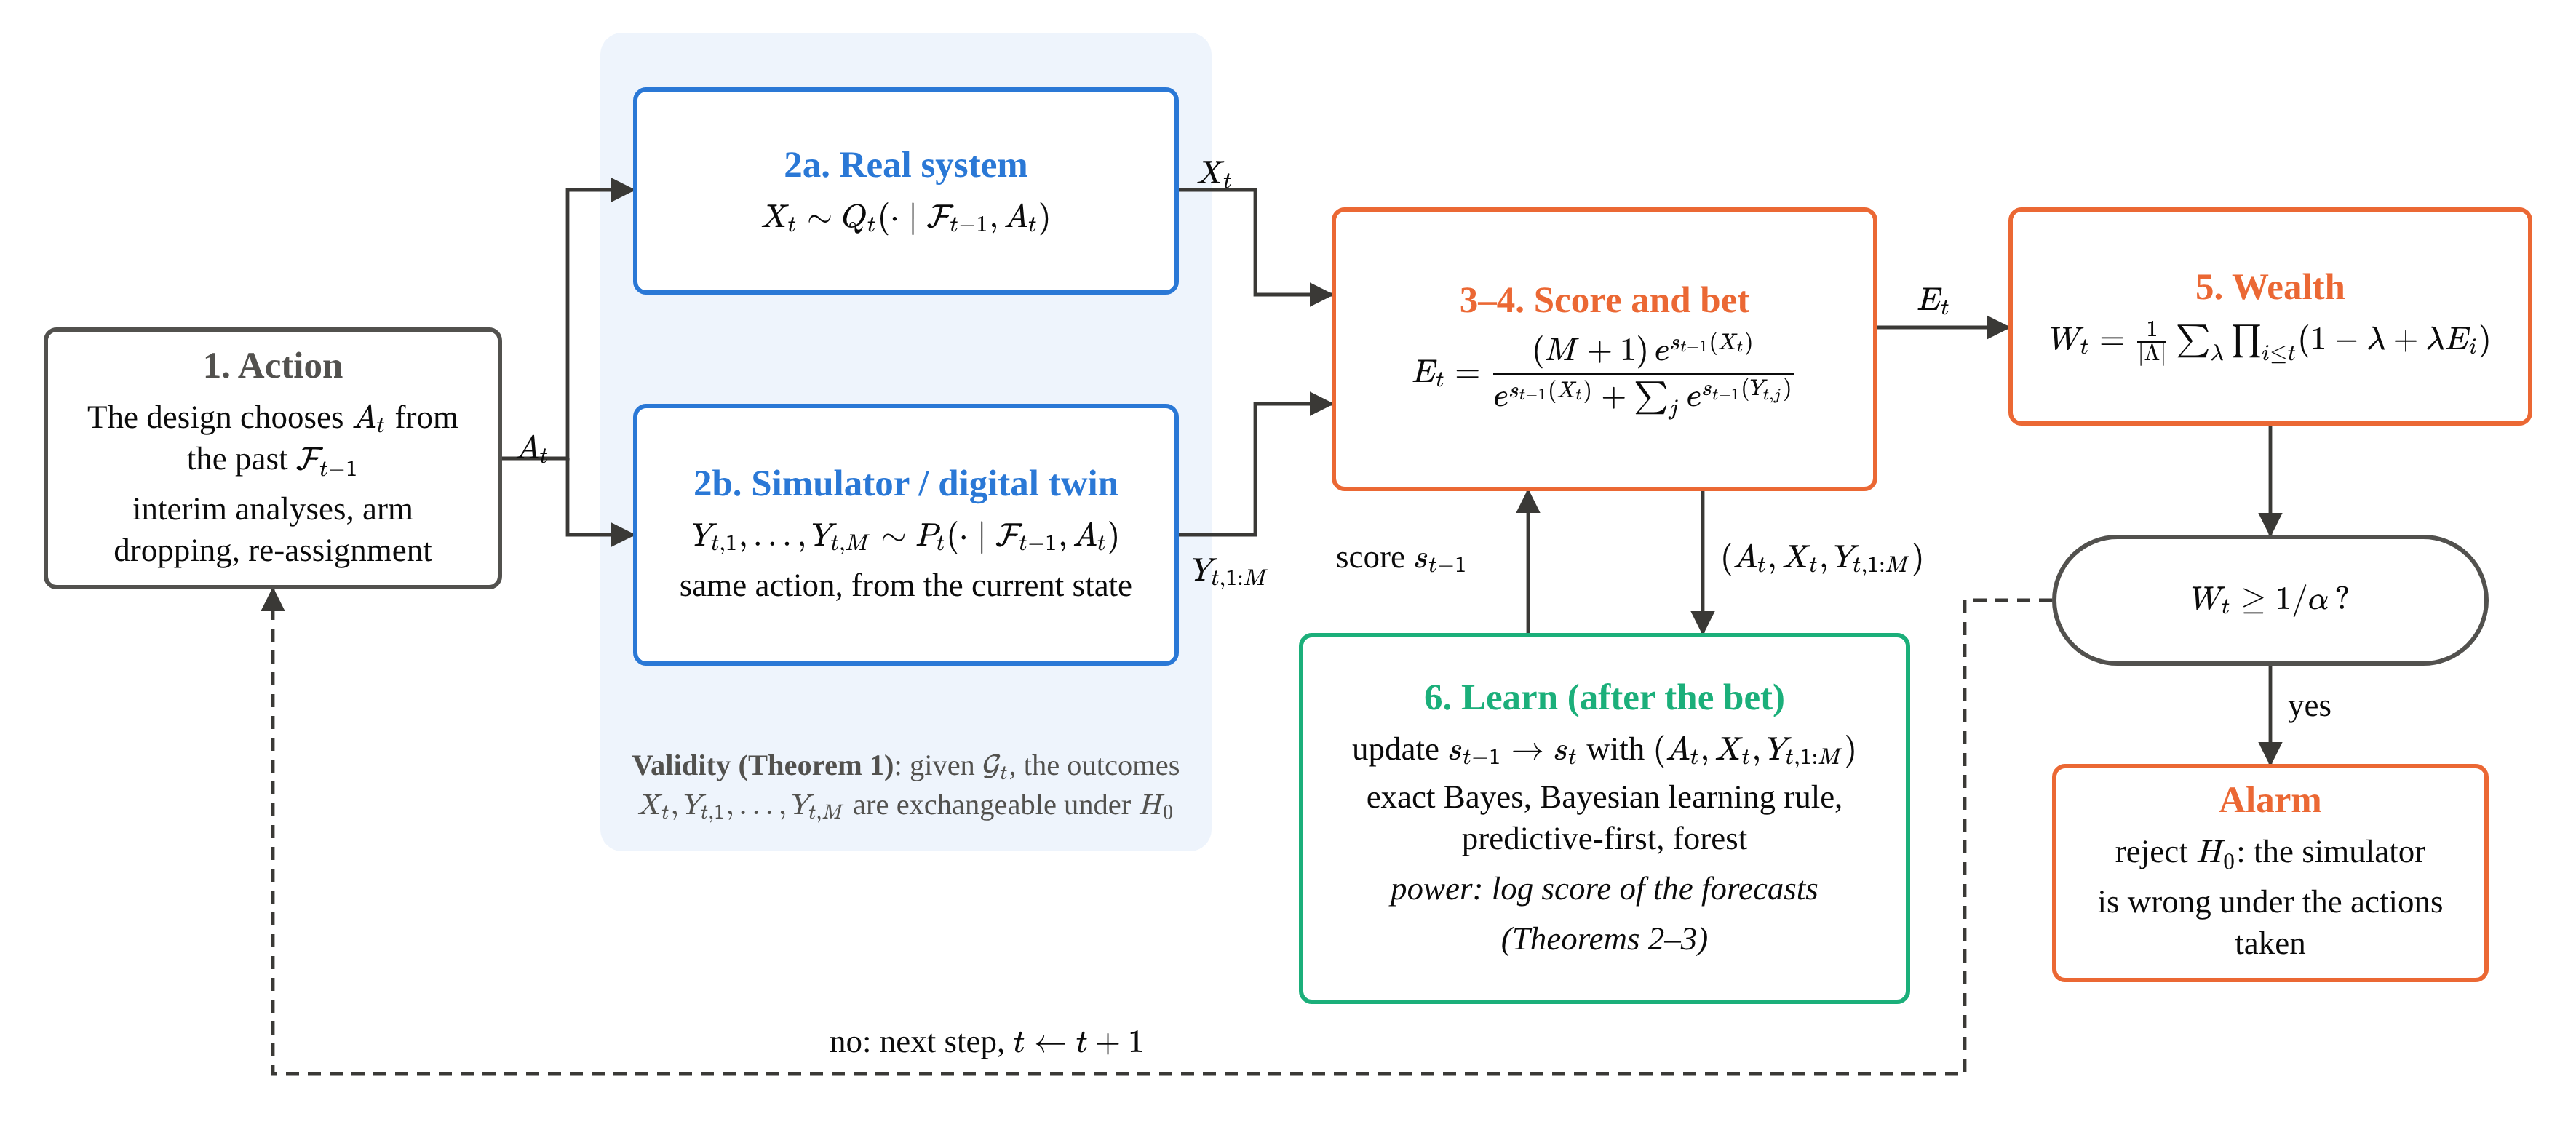
\includegraphics[width=\textwidth]{workflow.png}
\caption{One step of the procedure. The design chooses the action from the
past (1); the real system and the simulator are run under that action and
from the current state (2a, 2b); the current score, fixed before $X_t$ is
seen, turns the $M+1$ outcomes into the bet $E_t$ (3--4), which updates the
wealth (5); the null is rejected when the wealth reaches $1/\alpha$, and
otherwise the learner updates the score with the new outcomes (6) and the
next step begins. Validity rests on the shaded block alone; the learner
affects only power. Algorithm~1 (Section~\ref{sec:algorithm}) gives the
formulas of each step.}
\label{fig:workflow}
\end{figure}

%======================================================================
\section{Power: the growth rate}\label{sec:power}
%======================================================================

Validity is free; power is not. The time needed to reach $1/\alpha$ is governed
by the growth rate $\E[\log E_t \mid \G_t]$ \citep{grunwald2024safe}. Fix a
time, condition on $\G_t$ and drop the index. Let $P$ be the simulator law and
$Q$ the true law of the next outcome, with $Q \ll P$; let $T = e^{s}$ and
$Z = \E_P[T] < \infty$, and define the \emph{tilted null} $\tilde T$ by
$d\tilde T/dP = T/Z$, the exponential tilt of the simulator law by the score.
It is the alternative on which the score implicitly bets, and a perfect score
has $\tilde T = Q$. It is the \emph{forecast} of the score: not an estimate
of $Q$ but a deterministic function of the score, and we use the same symbol
$\tilde T$ for the law and its density. The letters for laws are fixed
throughout (Table~\ref{tab:notation}): $P$ for the simulator, $Q$ for the
truth, $\tilde T$ for the tilted null of a score $T$ and $m$ for a Bayesian
posterior predictive. Write $\rho = \E_Q[T]/Z$. Let $X \sim Q$
and, independently, $Y_1, \ldots, Y_M$ i.i.d.\ $P$, and let
$E^{(M)} = (M+1)T(X)/\{T(X) + \sum_{j} T(Y_j)\}$ be the factor \eqref{eq:mc}
computed from them. The \emph{growth rate} with $M$ simulator draws is
\begin{equation}\label{eq:growthrate}
\begin{aligned}
g_M = g_M(Q, P, T) &= \E_{Q \otimes P^M}\big[\log E^{(M)}\big] \\
&= \int \log\frac{(M+1)\,T(x)}{T(x) + \sum_{j=1}^M T(y_j)}\;
Q(dx) \prod_{j=1}^M P(dy_j),
\end{aligned}
\end{equation}
the expected logarithm of one factor when the whole wealth is bet. Since
$\log E^{(M)} \le \log(M+1)$ it is well defined in $[-\infty, \log(M+1)]$, and
finite when $s$ is bounded. It is at most zero when $Q = P$, by Jensen's
inequality and Proposition~\ref{prop:exact}. When a fraction $\lambda$ of the
wealth is bet, as in each term of \eqref{eq:wealth}, the rate is
\[
g_M(\lambda) = g_M(\lambda; Q, P, T)
= \E_{Q \otimes P^M}\big[\log(1 - \lambda + \lambda E^{(M)})\big],
\qquad g_M = g_M(1).
\]
In the sequential procedure $Q$, $P$ and $T$ are the conditional laws and the
score at time $t$, and the \emph{conditional growth rate}
$g_{M,t} = \E[\log E_t \mid \G_t]$ is $g_M$ evaluated at them; it is a
random variable that depends on the history. We write $g_M$ without arguments
when $Q$, $P$ and $T$ are clear from the context.

\begin{theorem}[Growth rate]\label{thm:growth}
Assume $\KL(Q\|P) < \infty$ and $\rho < \infty$.
\begin{enumerate}
  \item[(i)] (Ceiling.) $g_M \le \KL(Q\|P)$ for every $M$ and every score.
  \item[(ii)] (Unlimited budget.) As $M \to \infty$,
        $E^{(M)} \to (d\tilde T/dP)(X)$ almost surely, and if $s$ is bounded,
        $g_M \to g_\infty = \E_Q[\log (d\tilde T/dP)(X)] = \KL(Q\|P) - \KL(Q\|\tilde T)$.
  \item[(iii)] (Finite budget.) $g_M \ge g_\infty - \log\{1 + (\rho - 1)/(M+1)\}
        \ge g_\infty - (\rho - 1)/(M+1)$.
  \item[(iv)] (Local alternatives.) If $dQ/dP = 1 + \varepsilon \psi$ and
        $T = e^{\varepsilon h}$ with $\psi, h$ bounded and $\E_P[\psi] = 0$, and
        $\tilde h = h - \E_P[h]$, then
        $g_M = \frac{M}{M+1} \cdot \frac{\varepsilon^2}{2}
        \big(\E_P[\psi^2] - \E_P[(\psi - \tilde h)^2]\big) + O(\varepsilon^3)$,
        while $\KL(Q\|P) = \frac{\varepsilon^2}{2}\E_P[\psi^2] + O(\varepsilon^3)$.
\end{enumerate}
\end{theorem}

Part (i) is the log-optimality of the likelihood ratio. When the score is the
likelihood ratio, $\tilde T = Q$ and (ii) is the limit in Theorem~1 of
\citet{dombowsky2026besag}; part (iii) is their Theorem~3, rewritten with the
tilted null. The optimality of the likelihood-ratio score for every $M$ and the
finite-$M$ bound for that score were also obtained, concurrently, by
\citet[Proposition~3.2]{forre2026anytime} and
\citet[Proposition~4.2]{cortinovis2026slice}. What is new is the reading of an arbitrary score through
$\tilde T$ in (ii), and the local constant in (iv), which factorises the
efficiency relative to the oracle likelihood ratio into a simulation term and
a learning term,
\[
\frac{g_M}{\KL(Q\|P)} \approx
\underbrace{\frac{M}{M+1}}_{\text{simulation}} \times
\underbrace{\Big(1 - \frac{\KL(Q\|\tilde T)}{\KL(Q\|P)}\Big)}_{\text{learning}}.
\]
One draw per observation halves the growth rate and so roughly doubles the time
to detection; nine draws keep 90\% and sixteen 94\%. Away from the local regime,
$M/(M+1)$ is neither an upper nor a lower bound: for a large mean shift and a
perfect score the efficiency at $M = 1$ is lower, while an overconfident score
does better with a finite budget than with an infinite one, because
$E^{(M)} \le M+1$ truncates its bets (Section~\ref{sec:exp-budget}). This
complements \citet[Corollary~1]{dombowsky2026besag}, who show that the Monte
Carlo normalisation improves on an under-powered exact e-value. Over time,
the growth rates add up.

\begin{corollary}[Cumulative growth]\label{cor:cumulative}
For $\lambda \in \Lambda$ let
$g_{M,i}(\lambda) = \E[\log(1 - \lambda + \lambda E_i) \mid \G_i]$ be the
conditional growth rate of the $\lambda$-term of \eqref{eq:wealth} at time $i$.
\begin{enumerate}
\item[(i)] For every $\lambda \in \Lambda$ with $\lambda < 1$, and with no
condition on the scores,
$\log W_t \ge \sum_{i \le t} \log(1 - \lambda + \lambda E_i) - \log|\Lambda|$,
each increment lies in $[\log(1-\lambda),\, \log(1 + \lambda M)]$, and almost
surely
\[
\liminf_{t \to \infty} \frac1t \Big(\log W_t - \sum_{i \le t} g_{M,i}(\lambda)\Big) \ge 0 .
\]
\item[(ii)] If $1 \in \Lambda$ and the scores are bounded, $|s_t| \le B$, the
same holds for $\lambda = 1$, with increments $\log E_i \in [-2B, \log(M+1)]$
and rates $g_{M,i} = g_{M,i}(1)$.
\end{enumerate}
If, for some $\lambda \in \Lambda$, the average of $g_{M,i}(\lambda)$ over
$i \le t$ stays above $\bar g > 0$, the test rejects with probability one,
after about $(\log(1/\alpha) + \log|\Lambda|)/\bar g$ steps.
\end{corollary}

\begin{proof}
The average \eqref{eq:wealth} is at least $|\Lambda|^{-1}$ times any one of its
terms. Since $0 < E_i \le M+1$ by \eqref{eq:mc}, the increment
$\log(1 - \lambda + \lambda E_i)$ lies in $[\log(1-\lambda), \log(1+\lambda M)]$
for $\lambda < 1$, whatever the score; for $\lambda = 1$ and $|s_i| \le B$,
every term of \eqref{eq:mc} lies between $e^{-B}$ and $e^{B}$, so
$\log E_i \in [-2B, \log(M+1)]$. In both cases the differences
$\log(1 - \lambda + \lambda E_i) - g_{M,i}(\lambda)$ are bounded martingale
differences for the filtration $(\G_{i+1})$, and the martingale strong law
(Azuma--Hoeffding and Borel--Cantelli, as in the proof of
Proposition~\ref{prop:necessary}) shows that their average tends to zero
almost surely.
\end{proof}

Part (i) removes any assumption on the learner: the hedged terms of the
wealth have bounded increments for every score, so their growth is governed
by the conditional rates however the score is formed. The two rates are
related by concavity of the logarithm,
$\log(1 - \lambda + \lambda E) \ge \lambda \log E$, so
$g_{M,i}(\lambda) \ge \lambda\, g_{M,i}$: betting a fraction $\lambda$ keeps
at least a fraction $\lambda$ of the full growth rate, and more when the full
bet is too aggressive. Part (ii) needs bounded scores. Any predictable score
can be clipped to $[-B, B]$ without affecting validity
(Theorem~\ref{thm:valid}), and all our learners clip at $B = 30$, so (ii)
holds for them as implemented. Ridge penalisation alone does not provide such
a bound: with a fixed prior the penalised estimate is only guaranteed to satisfy
$\|\hat\theta_t\| = O(\sqrt{t})$ (compare the objective with its value at
$\theta = 0$), and unbounded features, such as polynomials of Gaussian outcomes,
make the score unbounded for any fixed coefficient.

The same theory gives the rate at which an action-ignoring twin produces a
false alarm. In the setting of Proposition~\ref{prop:necessary} the real
outcome has law $P_a$ and the simulator law is $\bar P$, so the factor is the
one Theorem~\ref{thm:growth} analyses with $Q = P_a$ and $P = \bar P$: under the
true null, the test behaves as if it were testing $P_a$ against $\bar P$.

\begin{corollary}[False-alarm rate of an action-ignoring twin]\label{cor:falsealarm}
In the setting of Proposition~\ref{prop:necessary}, suppose that the laws
$P_a$ and $\bar P$ and the score $T = e^{s}$, with $|s| \le B$, do not change
over time, that $\KL(P_a\|\bar P) < \infty$ for every action $a$, and that the
fraction of the first $t$ steps at which the policy plays $a$ converges to
$\varpi_a$. Let $g_M(a) = g_M(P_a, \bar P, T)$ be the growth rate
\eqref{eq:growthrate} with the real law $P_a$ in the role of $Q$ and the
simulator law $\bar P$ in the role of $P$, $g_\infty(a)$ its limit as
$M \to \infty$, and
$\tilde T_a = T\bar P/\E_{\bar P}[T]$. Then, under $H_0$:
\begin{enumerate}
\item[(i)] $g_\infty(a) = \KL(P_a\|\bar P) - \KL(P_a\|\tilde T_a)$ and
$g_M(a) \ge g_\infty(a) - (\rho_a - 1)/(M+1)$, where
$\rho_a = \E_{P_a}[T]/\E_{\bar P}[T]$ is the limit of
Proposition~\ref{prop:necessary}(i). If $1 \in \Lambda$, almost surely
$\liminf_t t^{-1}\log W_t \ge \sum_a \varpi_a\, g_M(a)$.
\item[(ii)] For every $\lambda$, every $M$ and every score,
$g_M(\lambda; P_a, \bar P, T) \le \KL(P_a\|\bar P)
\le \log\{1 + \chi^2(P_a\|\bar P)\}$, and almost surely
$\limsup_t t^{-1}\log W_t \le \sum_a \varpi_a \KL(P_a\|\bar P)$. The
likelihood-ratio score attains the bound as $M \to \infty$.
\item[(iii)] If the twin is run under randomised actions,
$\bar P = \sum_b u_b P_b$ with $u_b > 0$, then
$\KL(P_a\|\bar P) \le \log(1/u_a)$ and $\chi^2(P_a\|\bar P) \le 1/u_a - 1$;
with $K$ actions drawn uniformly, $\log K$ and $K - 1$.
\end{enumerate}
\end{corollary}

The proof is in Appendix~\ref{app:proofs}. The false alarm therefore arrives
after roughly $\log(1/\alpha)/\sum_a \varpi_a g_M(a)$ steps: the rate is a
Kullback--Leibler divergence, not the $\chi^2$ divergence that governs the
expected bet, and it is largest for a policy that concentrates on one action,
$\varpi_a \to 1$, as Thompson sampling does. The rate vanishes only if the arms
have the same law, and with $K$ arms it can never exceed $\log K$ per step.
Mathematically the corollary is Theorem~\ref{thm:growth} with the roles of the
laws reassigned, together with the standard bound for the redundancy of a
mixture code \citep{grunwald2007minimum}; its content is the reading.

%======================================================================
\section{Betting is predicting}\label{sec:predictive}
%======================================================================

Theorem~\ref{thm:growth} says what a good score is: one whose tilted null is
close to the truth. This section shows that choosing such a score is a problem
of sequential prediction, and gives update rules that solve it without
recomputation.

\subsection{The score as a one-step predictive}\label{sec:scores}

Fix a time $t$ and condition on $\G_t$, so that the action is known. Write
$p_t$ for the density of the simulator's next outcome under that action, and
$Q_t$, with density $q_t$, for the unknown law of the real next outcome. A score is a positive
function $T_t$ chosen from the past.

\paragraph{From scores to predictives.} Every score defines a probability
density for the next real outcome, its \emph{tilted null},
\begin{equation}\label{eq:tilt}
\tilde T_t(x) = \frac{T_t(x)\,p_t(x)}{Z_t},
\qquad
Z_t = \E_{P_t}[T_t] = \int T_t(x)\,p_t(x)\,dx,
\end{equation}
which integrates to one by construction. It is the simulator's density
reweighted by the score: the score raises the predicted density where
$T_t > Z_t$ and lowers it where $T_t < Z_t$. Conversely, for any predictive density of
the next real outcome computed from the past, the score equal to its ratio to
$p_t$ has $Z_t = 1$ and that density as its tilted null. The factor
\eqref{eq:mc} is unchanged when $T_t$ is multiplied by a positive constant,
$c\,T_t(X_t)/\sum_k c\,T_t(U_{t,k}) = T_t(X_t)/\sum_k T_t(U_{t,k})$, and so is
$\tilde T_t$. Scores up to a constant and predictive densities are therefore the
same object, and choosing a score means choosing a forecast of the next real
outcome. For example, with $p_t = \mathcal N(0,1)$, the linear score
$T_t(x) = e^{\theta x}$ gives $Z_t = e^{\theta^2/2}$ and
$\tilde T_t = \mathcal N(\theta, 1)$, a forecast that the real outcome is shifted
by $\theta$, and the quadratic score $T_t(x) = e^{-\gamma x^2/2}$ gives
$\tilde T_t = \mathcal N(0, 1/(1+\gamma))$, a forecast that it is less dispersed.

\paragraph{Only the ratio is needed.} The score is $q/p_t$, a ratio of two
densities, neither of which needs to be evaluated. A classifier separating
real outcomes (label 1) from simulator draws (label 0) estimates it: if the two
classes have prior weights $r$ and $1-r$, Bayes' theorem gives
\[
\Pr(\text{real} \mid x) = \frac{r\, q(x)}{r\, q(x) + (1-r)\, p_t(x)},
\qquad
\log\frac{\Pr(\text{real} \mid x)}{\Pr(\text{simulated} \mid x)}
= \log\frac{q(x)}{p_t(x)} + \log\frac{r}{1-r},
\]
so the classifier's logit is the log ratio up to an additive constant, which is
zero with balanced class weights \citep{thomas2022lfire} and in any case
cancels in \eqref{eq:mc}.

\paragraph{Why the Monte Carlo normalisation is needed.} Using the estimated
odds directly as the bet, $E^{\mathrm{plug}}_t = T_t(X_t)$ (the \emph{plug-in}),
has conditional mean $\E_{P_t}[T_t] = Z_t$ under the null, which is one only if
the estimated ratio integrates exactly to one against the simulator. A learned
ratio does not. If the estimated log ratio is the true one plus noise,
$\log T_t = \log(q/p_t) + \varepsilon$ with $\E[\varepsilon] = 0$, then
$\E[Z_t] = \E[e^{\varepsilon}] > 1$ by Jensen's inequality even when $q = p_t$:
noise in the learner alone makes the plug-in bets favourable on average under
the null, and their product grows. This is why an overfitted learner gives so
many false alarms (Section~\ref{sec:exp-drift}). The factor \eqref{eq:mc}
replaces the unknown $Z_t$ by its average over the real outcome and the $M$
simulations,
\[
E_t = \frac{T_t(X_t)}{\widehat Z_t},
\qquad
\widehat Z_t = \frac{1}{M+1}\Big\{T_t(X_t) + \sum_{j=1}^{M} T_t(Y_{t,j})\Big\},
\]
and Proposition~\ref{prop:exact} shows that this self-normalisation makes the
conditional mean exactly one under the null, whatever $Z_t$ is. For independent
data, \citet{forre2026anytime} fit the score by maximising the empirical growth
of this normalised bet on past observations; the update rules of
Sections~\ref{sec:simlik} and~\ref{sec:blr} replace that refit by one step per
observation, with a pathwise guarantee for the exact rule.

\paragraph{The wealth is a prequential likelihood ratio.} As $M \to \infty$,
$\widehat Z_t \to Z_t$ by the law of large numbers, so
$E_t \to T_t(X_t)/Z_t = \tilde T_t(X_t)/p_t(X_t)$ by \eqref{eq:tilt}. With the
betting fraction $\lambda = 1$, the log wealth therefore tends to
\begin{equation}\label{eq:prequential-wealth}
\log W_t \;=\; \sum_{i \le t} \log E_i \;\to\; \sum_{i \le t} \log \tilde T_i(X_i)
- \sum_{i \le t} \log p_i(X_i),
\end{equation}
the difference between the cumulative log scores of two forecasters, the
learned one $(\tilde T_i)$ and the simulator $(p_i)$, each forecast issued before
the outcome it is scored on. This is the prequential likelihood ratio of
\citet{dawid1984present}, and the monitor rejects at level $\alpha$ when the
learned forecaster has predicted the real outcomes $1/\alpha$ times better than
the simulator did. Under the truth $Q$ the expected increment is
\[
\E_Q\Big[\log\frac{f_i}{p_i}(X_i)\Big]
= \KL(Q\|P_i) - \KL(Q\|\tilde T_i),
\]
the information against the simulator minus the forecaster's own error, which
is Theorem~\ref{thm:growth}(ii); a finite $M$ multiplies it by about
$M/(M+1)$ (Theorem~\ref{thm:growth}(iv)). Validity comes from exchangeability;
power is a matter of prediction.

\paragraph{Predictive updating.} This is the point of view of the predictive
approach to Bayesian inference. In a Bayesian model with likelihood $q_\theta$
and prior $\pi_0$, the forecasts are the one-step posterior predictives
\[
m_t(x) = \int q_\theta(x \mid x_{1:t-1})\,\pi_{t-1}(d\theta),
\qquad
\pi_{t-1}(d\theta) \propto \prod_{i<t} q_\theta(x_i \mid x_{1:i-1})\,\pi_0(d\theta),
\]
and by the chain rule \eqref{eq:prequential} they determine the joint law of
the observations; for exchangeable sequences de Finetti's theorem recovers the
prior and the likelihood from them. \citet{fong2023martingale} take the
predictives as the primitive. One specifies an update rule
\[
m_{t+1} = \mathcal U_t(m_t, X_t),
\]
and recovers posterior uncertainty by \emph{predictive resampling}: draw
$X_{t+1} \sim m_{t+1}$, update, draw $X_{t+2} \sim q_{t+2}$, and so on; any
quantity computed from the limiting predictive is then a draw from the
\emph{martingale posterior}. The imputation converges when the predictives form
a martingale,
\[
\E_{X \sim m_t}\big[\mathcal U_t(m_t, X)(x)\big] = m_t(x) \quad \text{for all } x,
\]
that is, when imputing one more outcome does not move the forecast on average;
such sequences are the conditionally identically distributed sequences of
\citet{berti2004limit}, and Bayesian predictives satisfy the condition. The
monitor uses only the first half of this construction, the rule
$\mathcal U_t$ that turns the current forecast and a new outcome into the next
forecast, and never imputes. The rule must satisfy four requirements.
\begin{enumerate}
  \item It must be sequential: the bet on $X_t$ is fixed before $X_t$ is seen,
        so the forecast cannot be refitted on data that include $X_t$.
  \item It should forecast well one step ahead, since by
        \eqref{eq:prequential-wealth} the growth of the wealth is the one-step
        log score of the forecasts.
  \item It should hedge early on: an overconfident forecast can lose all the
        growth (Theorem~\ref{thm:growth}), and averaging over what has not yet
        been learned protects against it.
  \item It must be computable from simulations alone, since $p_t$ is
        available only as a sampler.
\end{enumerate}
The rest of the section looks for such a rule. Bayes' theorem is the natural
first candidate: it is optimal for the log score and gives the Bayes factor
(Section~\ref{sec:exactbayes}), but it violates the fourth requirement,
because its normalising constant is an integral against $p_t$. The
simulation likelihood (Section~\ref{sec:simlik}) restores it by putting the
Monte Carlo normalisation of \eqref{eq:mc} inside the likelihood, and
Section~\ref{sec:blr} gives one-step approximations that meet the first
requirement at a fixed cost per observation.

\subsection{The Bayesian update rule}\label{sec:exactbayes}

By \eqref{eq:prequential-wealth}, the monitor is paid the log score of its
forecasts $\tilde T_t$. Which forecast should it issue? If the real outcomes
are described by a model $\{Q_\theta\}$ with prior $\pi_0$, the answer is the
Bayesian rule: $\mathcal U_t$ is Bayes' theorem, the forecast is the posterior
predictive $m_t$, and the score is $T_t = m_t/p_t$, whose tilted null
\eqref{eq:tilt} is $m_t$ itself, with $Z_t = 1$. Because the logarithmic score
is strictly proper, this is the best bet on average under the model.

\begin{proposition}[The posterior predictive is the Bayes-optimal bet]\label{prop:bayesopt}
Let $\{Q_\theta\}$ be a model with prior $\pi_0$, under which, given $\theta$,
the outcomes are i.i.d.\ $Q_\theta$ given the past and the action, and let $m_t$
be the posterior predictive density of $X_t$ given $\G_t$. For every
$\G_t$-measurable score $T$ with $\E_P[T] < \infty$, the Bayes-expected growth
satisfies
\[
\E\big[\log E_t^\infty \mid \G_t\big] \le
\E\Big[\log \frac{m_t}{p}(X_t) \Bigm| \G_t\Big]
\quad \text{under the Bayesian model,}
\]
with equality if and only if $T \propto m_t/p$, $P$-almost everywhere.
\end{proposition}

\begin{proof}
$E_t^\infty = \tilde T(X_t)/p(X_t)$, where $\tilde T = T p/\E_P[T]$ is a
density. Under the Bayesian model, $X_t$ given $\G_t$ has density $m_t$, so
the difference between the two sides is
$\E_{m_t}[\log (\tilde T/m_t)] = -\KL(m_t\|\tilde T) \le 0$.
\end{proof}

Which model? Section~\ref{sec:scores} already supplies one. A log-linear
score $s = \theta^\top\phi$ has the tilted null \eqref{eq:tilt}
$dQ_\theta/dP = \exp\{\theta^\top \phi(x) - \log Z(\theta)\}$, with
$Z(\theta) = \E_P[e^{\theta^\top\phi}]$, and as $\theta$
varies these tilted nulls form an exponential family built on the simulator.
Taking this family as the model for the real outcomes means that the forecast
is an average of tilted nulls, $m_t = \int q_\theta\, \pi_{t-1}(d\theta)$, and
its score $T_t = \int (dQ_\theta/dP)\, \pi_{t-1}(d\theta)$ turns the process into
a Bayes factor.

\begin{proposition}[Predictive scores give the Bayes factor]\label{prop:bayes}
With this score $\E_P[T_t] = 1$, the unlimited-budget factor is
$E_t^\infty = T_t(X_t)$, and
$\prod_{i\le t} E_i^\infty = \int \prod_{i \le t} (dQ_\theta/dP)(X_i)\,\pi_0(d\theta)$,
the Bayes factor of the tilted family against the simulator. For i.i.d.\ data
and under the usual regularity conditions for Laplace approximations, its
logarithm is $\sup_\theta \sum_{i\le t}\log (dQ_\theta/dP)(X_i) - \frac{d}{2}\log t
+ O_P(1)$, and $t^{-1}$ times it converges to
$\KL(Q\|P) - \inf_\theta \KL(Q\|Q_\theta)$.
\end{proposition}

\begin{proof}
$\E_P[dQ_\theta/dP] = 1$ for every $\theta$. The product of one-step predictive
ratios is the ratio of marginal likelihoods, and the expansion is the
Laplace approximation of \citet{clarke1990information}; see
Appendix~\ref{app:proofs}.
\end{proof}

With posterior predictive scores the learning penalty is paid once,
$(d/2)\log t$ in total, whereas a plug-in estimate bets everything on one tilt
and can lose all its growth.

Computing a Bayes factor as a product of one-step posterior predictives, as in
\eqref{eq:prequential}, is classical, and it appears in several equivalent
forms. In Dawid's prequential form \citep{dawid1984present}, the log marginal
likelihood is the cumulative log score of the forecasts $m_i$, each issued
before $x_i$ is seen,
\[
\log m(x_{1:t}) = \sum_{i=1}^{t} \log m_i(x_i),
\qquad
m_i(x) = \int q_\theta(x \mid x_{1:i-1})\,\pi_{i-1}(d\theta).
\]
In minimum description length, $-\log m(x_{1:t}) = \sum_i \{-\log m_i(x_i)\}$
is the length of the Bayes universal code, the sum of the lengths of the
predictive codes \citep{rissanen1984universal,grunwald2007minimum}, and its
regret against the best code in the model is
\[
-\log m(x_{1:t}) - \inf_\theta \Big\{-\sum_{i \le t}\log q_\theta(x_i \mid x_{1:i-1})\Big\}
= \frac d2 \log t + O_P(1)
\]
for i.i.d.\ data under regularity conditions \citep{clarke1990information}.
In sequential Monte Carlo, the evidence is estimated by the same product: with
particles $\theta^{(k)}$ and normalised weights $\omega_{i-1}^{(k)}$ approximating
$\pi_{i-1}$,
\[
\tilde m_i(x_i) = \sum_{k} \omega_{i-1}^{(k)}\, q_{\theta^{(k)}}(x_i \mid x_{1:i-1}),
\qquad
\tilde m(x_{1:t}) = \prod_{i=1}^{t} \tilde m_i(x_i),
\]
and the particles are reweighted by $q_{\theta^{(k)}}(x_i \mid x_{1:i-1})$ and
resampled as each observation arrives \citep{kong1994sequential,chopin2002sequential}.
Finally, for exchangeable models, averaging the chain rule over all orderings of
the observations gives
\[
\log m(x_{1:t}) = \sum_{k=0}^{t-1} \binom{t}{k}^{-1} \sum_{|S| = k}
\frac{1}{t-k} \sum_{j \notin S} \log m(x_j \mid x_S),
\]
where $m(\cdot \mid x_S)$ is the posterior predictive given the observations in
$S$: the log marginal likelihood is the sum, over training-set sizes, of
exhaustive leave-$(t-k)$-out cross-validation scores \citep{fong2020marginal}.
All these forms need the predictive density $m_i$, and hence the normalising
constant of the model. Section~\ref{sec:simlik} gives the analogue of the
product for a model that can only be sampled, and the averages over posterior
nodes used to compute it in Section~\ref{sec:blr} are of the same form as the
sequential Monte Carlo estimate $\tilde m_i$. Proposition~\ref{prop:bayes} is, however, only a
benchmark: Bayes' rule for the tilt needs $Z(\theta)$ at every
step and for every $\theta$. This is the normalising constant of
\eqref{eq:tilt} that the plug-in bet cannot know (Section~\ref{sec:scores}),
an integral against a law that can only be sampled, and it is exactly what the
Monte Carlo factor estimates from the $M+1$ outcomes. The next section uses
that estimate inside the likelihood.

\subsection{The simulation likelihood}\label{sec:simlik}

The Monte Carlo factor itself provides the way out. Fix a parameter
$\theta \in \mathbb{R}^d$ and $\G_t$-measurable features $\phi_t$, write
$U_{t,0} = X_t$ and $U_{t,k} = Y_{t,k}$, and let
\[
E_t(\theta) = \frac{(M+1)\exp\{\theta^\top\phi_t(U_{t,0})\}}
{\sum_{k=0}^{M}\exp\{\theta^\top\phi_t(U_{t,k})\}}
\]
be the factor \eqref{eq:mc} with score $s_t = \theta^\top\phi_t$. Up to the
constant $M+1$, $E_t(\theta)$ is the probability that a conditional-logit model
of the question ``which of the $M+1$ outcomes is the real one?'' assigns to the
real outcome. It is a likelihood for $\theta$ whose normalising constant is a
sum over the simulations, and it is always computable. We call
$L_t(\theta) = \prod_{i \le t} E_i(\theta)$ the \emph{simulation likelihood}.
Its logarithm is, up to constants, the InfoNCE objective of contrastive
learning \citep{oord2018representation}, a link also drawn by
\citet{cortinovis2026slice} for the optimal score, and the partial likelihood of
ranking-based noise-contrastive estimation \citep{ma2018noise}. With a prior
$\pi_0$ on $\theta$ and posterior $\pi_t \propto \pi_0 L_t$, the
\emph{posterior-predictive bet} is
$\bar E_t = \int E_t(\theta)\, \pi_{t-1}(d\theta)$. This posterior,
$\pi_t(\theta) \propto \pi_0(\theta)\exp\{-\sum_{i \le t}\ell_i(\theta)\}$ with
$\ell_i = -\log E_i$, is a prequential posterior in the sense of
\citet{sinharoy2026prequential}, who update generalised posteriors of
simulator-based forecasting models with a one-step-ahead loss estimated from
simulations; the particular loss $-\log E_t(\theta)$, with learning rate one,
is what makes the posterior mixture of the bets an e-process
(Theorem~\ref{thm:simlik}(i)).

\begin{theorem}[Predictive updating on the simulation likelihood]\label{thm:simlik}
Suppose the conditions of Theorem~\ref{thm:valid} hold for each fixed $\theta$
(simulations under the action taken, $\phi_t$ $\G_t$-measurable), that
$\|\phi_t\| \le G$, and that $\pi_0$ is the uniform distribution on a convex
compact set $\Theta \subset \mathbb{R}^d$ with nonempty interior and diameter
at most $2D$.
\begin{enumerate}
  \item[(i)] (Exact factorisation and validity.) The wealth
        $\bar W_t = \prod_{i \le t} \bar E_i$ equals
        $\int L_t(\theta)\,\pi_0(d\theta)$. It is a test martingale under
        $H_0$, for every policy, and it is updated by one posterior step per
        observation, with no recomputation.
  \item[(ii)] (Pathwise regret.) On every sample path, for every
        $t \ge d/(4GD)$,
        \[
        \log \bar W_t \;\ge\; \sup_{\theta \in \Theta} \log L_t(\theta)
        - d \log t - d \log\frac{4eGD}{d}.
        \]
        If the maximiser $\theta^*_t$ of $L_t$ lies in $\Theta$ at distance at
        least $r_t = \sqrt{d/(tG^2)}$ from its boundary, the bound improves to
        $\log \bar W_t \ge \log L_t(\theta_t^*) - \frac d2 \log t
        - \frac d2 \log\frac{e G^2 (2D)^2}{d}$.
  \item[(iii)] (Growth.) Let $g_{M,i}(\theta) = \E[\log E_i(\theta) \mid \G_i]$,
        the conditional growth rate \eqref{eq:growthrate} of the fixed score
        $T = e^{\theta^\top\phi}$, and $g_M(\theta) = g_M(Q, P, e^{\theta^\top\phi})$.
        For every $\theta \in \Theta$, almost surely,
        \[
        \liminf_{t \to \infty} \frac1t \Big(\log \bar W_t - \sum_{i \le t} g_{M,i}(\theta)\Big) \ge 0 .
        \]
        In particular, for i.i.d.\ data under a fixed action and features,
        $\liminf_t t^{-1}\log \bar W_t \ge \sup_{\theta\in\Theta} g_M(\theta)$,
        and, if $\KL(Q\|P) < \infty$, by Theorem~\ref{thm:growth}
        $g_M(\theta) \ge \KL(Q\|P) - \KL(Q\|Q_\theta) - \log\{1 + (\rho_\theta - 1)/(M+1)\}$,
        where $Q_\theta$ is the tilt of $P$ by $\theta^\top\phi$ and
        $\rho_\theta = \E_Q[e^{\theta^\top\phi}]/\E_P[e^{\theta^\top\phi}]$.
\end{enumerate}
\end{theorem}

Part (i) says that exact Bayesian updating is available once the likelihood is
the right one: not the likelihood of the real outcome under the tilt, which
needs $Z(\theta)$, but the likelihood of the real outcome's position among the
simulations, which the simulations normalise. The Bayes factor of
Proposition~\ref{prop:bayes} is its limit as $M \to \infty$. Part (ii) holds on
every path, with no assumption on the alternative: the monitor is never more
than $d\log t$ behind the best fixed score in the class chosen in hindsight,
the same simulations included. The argument is the standard one for Bayesian mixtures
of log-concave likelihoods \citep{kakade2005online,grunwald2007minimum},
applied to the simulation likelihood, whose log is concave in $\theta$ and
whose gradient is bounded by $2G$. Part (iii) turns this into growth at the rate of
the best tilt in the class, up to the simulation cost of
Theorem~\ref{thm:growth}(iii), and Ville's inequality then gives rejection
after about $\{\log(1/\alpha) + d\log t\}/\sup_\theta g_M(\theta)$ steps.

\subsection{Approximate posteriors and the Bayesian learning rule}\label{sec:blr}

The integral in $\bar E_t$ is over $\theta$ only, and any $\G_t$-measurable
distribution $\nu_{t-1}$ on $\theta$, an approximate posterior, in
place of $\pi_{t-1}$ still gives a valid bet
$E^{\nu}_t = \int E_t(\theta)\,\nu_{t-1}(d\theta)$, because $E_t(\theta)$ is fair
for each $\theta$. The price of the approximation is bounded as follows.

\begin{proposition}[Approximate predictive bets]\label{prop:approx}
Let $\nu_{t-1}$ be any $\G_t$-measurable distribution on $\mathbb{R}^d$ with mean
$\bar\theta_{t-1}$ and covariance $\Sigma_{t-1}$, and $\|\phi_t\| \le G$. Then
$E^{\nu}_t$ is an e-value given $\G_t$, and
\[
\log E^{\nu}_t \;\ge\; \E_{\nu_{t-1}}\big[\log E_t(\theta)\big]
\;\ge\; \log E_t(\bar\theta_{t-1}) - \frac{G^2}{2}\,\mathrm{tr}\,\Sigma_{t-1}.
\]
\end{proposition}

\begin{proof}
Validity follows from Fubini's theorem. The first inequality is Jensen's.
The function $\theta \mapsto \log E_t(\theta)$ is concave, with gradient
$\phi_t(U_{t,0}) - \sum_k w_k \phi_t(U_{t,k})$ and Hessian
$-\mathrm{Cov}_w(\phi_t)$, where $w_k \propto e^{\theta^\top\phi_t(U_{t,k})}$;
since $\mathrm{Cov}_w(\phi_t) \preceq \E_w[\phi_t\phi_t^\top] \preceq G^2 I$,
Taylor's theorem with integral remainder around $m = \bar\theta_{t-1}$ gives
$\log E_t(\theta) \ge \log E_t(m) + \nabla\log E_t(m)^\top(\theta - m)
- \frac{G^2}{2}\|\theta - m\|^2$ for every $\theta$. Taking the expectation
under $\nu_{t-1}$, the linear term vanishes because $m$ is its mean, and
$\E_{\nu_{t-1}}\|\theta - m\|^2 = \mathrm{tr}\,\Sigma_{t-1}$.
\end{proof}

A predictive bet built from an approximate posterior is therefore never worse
than the plug-in bet at its mean by more than
$\frac{G^2}{2}\sum_i \mathrm{tr}\,\Sigma_{i-1}$. If the posterior precision grows
at least linearly, $\Sigma_i^{-1} \succeq \Sigma_0^{-1} + i\,\gamma I$ for some
$\gamma > 0$, this is at most $\frac{G^2 d}{2\gamma}\log t + O(1)$, the order of
the regret in Theorem~\ref{thm:simlik}; the constant degrades when the
features are nearly collinear under the simulator, so that $\gamma$ is small. The Bayesian learning rule \citep{khan2023bayesian}
provides such a posterior. It approximates a posterior within an exponential
family by natural-gradient descent on the expected loss plus the Kullback--Leibler
divergence from the prior; in a stream, one step per observation with the
previous approximation as the prior \citep{jones2024bong} gives, for a Gaussian
$\nu_t = \mathcal N(\bar\theta_t, S_t^{-1})$ and a per-step loss $\ell_t$,
\begin{equation}\label{eq:blr}
S_t = S_{t-1} + \E_{\nu_{t-1}}[\nabla^2 \ell_t], \qquad
\bar\theta_t = \bar\theta_{t-1} - S_t^{-1}\, \E_{\nu_{t-1}}[\nabla \ell_t],
\end{equation}
which is exact Bayesian updating (the Kalman filter) for a Gaussian likelihood
and one step of online Newton in general. Its cost is $O((M+1)d^2)$ per step,
with no refitting and no burn-in.

Two losses are natural. On the simulation
likelihood, $\ell_t(\theta) = -\log E_t(\theta)$, with gradient
$\sum_k w_k \phi_t(U_{t,k}) - \phi_t(U_{t,0})$ and Hessian
$\mathrm{Cov}_w(\phi_t)$; expectations under $\nu_{t-1}$ are computed with fixed
antithetic nodes, and the bet is the average of $E_t(\theta)$ over the nodes,
so Theorem~\ref{thm:simlik} and Proposition~\ref{prop:approx} apply directly.
Alternatively, $\ell_t$ is the balanced logistic loss of classifying the real
outcome (weight one) against the $M$ simulations (weight $1/M$ each), a
generalised posterior \citep{bissiri2016general,sinharoy2026prequential} that identifies the same tilt
through noise-contrastive estimation \citep{gutmann2012noise}; with the probit
approximation $\E_\nu[\sigma(z^\top\theta)] \approx \sigma(\kappa\bar\eta)$,
$\bar\eta = z^\top\bar\theta$, $v = z^\top S^{-1}z$ and $\kappa = (1+\pi v/8)^{-1/2}$, the
score is the predictive log-odds $\kappa\bar\eta$ and is inserted in \eqref{eq:mc}.
Both scores start at zero, so the monitor starts by not betting, and both
shrink where the posterior is uncertain. Features are standardised with
simulator draws only, before any real data are seen, so that the score stays
predictable.

The same two classifiers can also be updated without a posterior over their
weights, by updating their predictive directly, as martingale posteriors do
\citep{fong2023martingale}. The learner then carries the predictive itself,
$\sigma(z^\top\theta_t)$ for the logistic loss or the softmax
$e^{\theta_t^\top z_k}/\sum_{k'} e^{\theta_t^\top z_{k'}}$ over the $M+1$
outcomes for the simulation likelihood, and updates it by Fisher scoring on the
predictive's own log-likelihood,
\begin{equation}\label{eq:mp}
I_t = I_{t-1} + J_t(\theta_{t-1}), \qquad
\theta_t = \theta_{t-1} - I_t^{-1}\, \nabla_t(\theta_{t-1}),
\end{equation}
where $\nabla_t$ is the gradient of the new batch's loss and $J_t$ its Fisher information,
which for both losses does not depend on the labels, and $I_0$ is a prior
precision. Under the predictive the gradient has mean zero, so $\theta_t$ is a
martingale, which is the condition for the convergence of predictive resampling
in parametric martingale posteriors \citep{fong2023martingale}; the predictive
$\sigma(z^\top\theta_t)$, a nonlinear function of $\theta_t$, is a martingale
only to first order in the step $I_t^{-1}\nabla_t$. The
bet uses either the current predictive (the \emph{plug-in predictive}) or an
average of the factor over $N$ \emph{predictive-resampling} paths, obtained by
running \eqref{eq:mp} forward from $(\theta_{t-1}, I_{t-1})$ on past batches
whose labels are drawn from the predictive; this is the martingale posterior's
uncertainty, truncated at $h_{\max}$ steps ($N = 16$, $h_{\max} = \min(t, 200)$, refreshed every
ten steps). The two routes differ in where uncertainty comes from: a Gaussian
approximation of a posterior, or simulation from the predictive. Both give valid
bets.

The predictive rule need not be parametric. The simplest rule of
\citet{fong2023martingale} is the empirical predictive, under which the next
observation is a copy of a past one, $\mathbb P_{n+1} = (n\mathbb P_n + \delta_{x_{n+1}})/(n+1)$;
predictive resampling with it is a P\'olya urn, and its martingale posterior is
the Bayesian bootstrap, which reweights the data by
$\mathrm{Dirichlet}(1, \ldots, 1)$ weights. Any learner can therefore be made a
martingale-posterior learner. We do this for a random forest: the exchangeable
units are the monitoring steps, each contributing its real outcome (label one,
weight one) and its $M$ simulations (label zero, weight $1/M$), and each of $N$
trees is fitted to the past steps with its own Dirichlet weights, so that the
forest is a sample from the martingale posterior. A leaf's score is its
log-odds under a $\mathrm{Beta}(a, a)$ prior on its weighted class counts,
$\log\{(w_1 + a)/(w_0 + a)\}$, so that leaves supported by little data bet
little, and the bet is the posterior-predictive mixture
$\bar E_t = N^{-1}\sum_b E_t(\mathrm{tree}_b)$, as in Theorem~\ref{thm:simlik};
each tree is fitted on the past only, so the mixture is exactly fair, and the
first inequality of Proposition~\ref{prop:approx} applies. The trees are
refitted every few steps ($N = 16$, depth at most 6, $a = 3$).

Under a Gaussian posterior the logit could also be scored on the
ratio scale, $\log\E_\nu[e^{z^\top\theta}] = \bar\eta + v/2$, which is the predictive
of Propositions~\ref{prop:bayesopt} and~\ref{prop:bayes} when the posterior is
exact; its uncertainty premium $v/2$ over-bets where the approximation is least
reliable, and it is the worst score in every experiment below. If the system
may drift, replacing $S_{t-1}$ by $\gamma S_{t-1}$, $\gamma < 1$, before each
update keeps the monitor responsive, and like every choice of score leaves
validity untouched.

\subsection{The method in full}\label{sec:algorithm}

The pieces of this section fit together as follows, for the default score, the
logistic Bayesian learning rule with the probability-scale predictive; the
steps are numbered as in Figure~\ref{fig:workflow}. Each step is followed by
the role it plays.

\paragraph{Algorithm 1 (Monte Carlo e-process with a predictive score).}
\textbf{Input:} a simulator that can be run under any action from any state; a
feature map $z(x)$; the number of simulations $M$; the level $\alpha$; the grid
$\Lambda$ of betting fractions. \textbf{Initialise:} standardise $z$ with
simulator draws only; set $\bar\theta_0 = 0$, $S_0 = I$ (vaguer on the intercept), and
$W_0 = 1$.
\begin{enumerate}
  \item \textbf{Action.} Observe the action $A_t$ chosen by the design from the
        past (arm, prompt, dose). --- It defines the null law $P_t$.
  \item \textbf{Simulate.} Draw $Y_{t,1}, \ldots, Y_{t,M}$ from the simulator
        under $A_t$ from the current state, and observe $X_t$.
        --- Exchangeable with $X_t$ under $H_0$.
  \item \textbf{Score.} For each of the $M+1$ outcomes $x$, compute
        \[
        \begin{gathered}
        \bar\eta = z(x)^\top \bar\theta_{t-1}, \qquad v = z(x)^\top S_{t-1}^{-1} z(x), \\
        \kappa = (1 + \pi v/8)^{-1/2}, \qquad
        s_{t-1}(x) = \mathrm{clip}(\kappa\,\bar\eta,\, -B,\, B) .
        \end{gathered}
        \]
        --- $s_{t-1}$ is the predictive log-odds of ``real'' against
        ``simulated'', an estimate of $\log(q/p)$ shrunk where the posterior is
        uncertain; it forecasts $\tilde T_t \propto p_t\, e^{s_{t-1}}$
        \eqref{eq:tilt}. Clipping at $B$ (we use $B = 30$) keeps the score
        predictable, so validity is unaffected, and makes
        Corollary~\ref{cor:cumulative}(ii) apply.
  \item \textbf{Bet.}
        \[
        E_t = \frac{(M+1)\, e^{s_{t-1}(X_t)}}{e^{s_{t-1}(X_t)} + \sum_{j=1}^{M} e^{s_{t-1}(Y_{t,j})}} .
        \]
        --- Exactly fair under $H_0$ (Theorem~\ref{thm:valid}); close to
        $\tilde T_t(X_t)/p_t(X_t)$ for large $M$.
  \item \textbf{Wealth.} $W_t = |\Lambda|^{-1}\sum_{\lambda\in\Lambda}
        \prod_{i\le t}(1-\lambda+\lambda E_i)$; reject $H_0$ when
        $W_t \ge 1/\alpha$. --- A test martingale; its log is the
        prequential likelihood ratio \eqref{eq:prequential-wealth} of the
        forecasts against the simulator, and it grows at about
        $\frac{M}{M+1}\{\KL(Q\|P) - \KL(Q\|\tilde T)\}$ per step
        (Theorem~\ref{thm:growth}).
  \item \textbf{Learn.} Only now, with labels $y_0 = 1$ for $X_t$ and $y_j = 0$
        for $Y_{t,j}$, weights $w_0 = 1$ and $w_j = 1/M$, and
        $p_k = \sigma(s_{t-1}(U_{t,k}))$, update
        \[
        \begin{gathered}
        \nabla_t = \sum_{k=0}^{M} w_k (p_k - y_k)\, z_k, \qquad
        J_t = \sum_{k=0}^{M} w_k \kappa_k\, p_k (1 - p_k)\, z_k z_k^\top, \\
        S_t = S_{t-1} + J_t, \qquad \bar\theta_t = \bar\theta_{t-1} - S_t^{-1} \nabla_t .
        \end{gathered}
        \]
        --- One step of the Bayesian learning rule \eqref{eq:blr}; the score
        stays predictable.
\end{enumerate}
\textbf{Variants.} With the simulation likelihood (Section~\ref{sec:simlik}),
steps 3--4 are replaced by the posterior-predictive mixture
$\bar E_t = N^{-1}\sum_b E_t(\theta_b)$ over posterior nodes $\theta_b$, and step 6
by \eqref{eq:blr} with $\ell_t = -\log E_t(\theta)$; Theorem~\ref{thm:simlik} and
Proposition~\ref{prop:approx} then apply.

\textbf{Predictive-first version.} The score can also be updated without any
posterior over $\theta$, by carrying and updating the classifier's predictive
itself, $c_t(x) = \sigma(z(x)^\top\theta_t)$, as martingale posteriors do.
Steps 3 and 6 then become
\[
\text{3'.}\quad s_{t-1}(x) = z(x)^\top\theta_{t-1} = \log\frac{c_{t-1}(x)}{1 - c_{t-1}(x)},
\]
\[
\text{6'.}\quad
I_t = I_{t-1} + \sum_{k=0}^{M} w_k\, p_k(1-p_k)\, z_k z_k^\top, \qquad
\theta_t = \theta_{t-1} + I_t^{-1}\sum_{k=0}^{M} w_k\,(y_k - p_k)\, z_k,
\]
with $p_k = c_{t-1}(U_{t,k})$ and $I_0 = S_0$: Fisher scoring on the
predictive's own log-likelihood \eqref{eq:mp}, under which $\theta_t$ is a martingale.
The forecast is then $\tilde T_t \propto p_t\, c_{t-1}/(1-c_{t-1})$, the
current predictive odds with no shrinkage. To carry uncertainty without a
posterior, step 4 averages the factor over $N$ predictive-resampling paths
$\theta^{(b)}$, obtained by running 6' forward from $(\theta_{t-1}, I_{t-1})$ on
past batches whose labels are drawn from the predictive,
$\bar E_t = N^{-1}\sum_b E_t(\theta^{(b)})$. For the logistic loss, 6' is the
Newton step of 6 taken at the point $\theta_{t-1}$ rather than averaged over a
Gaussian posterior: the two versions differ only in where uncertainty comes
from, a Gaussian approximation ($\kappa$ in step 3) or simulation from the
predictive (the paths in step 4). With a random forest under the empirical
predictive, step 3 uses the trees' leaf log-odds, step 4 averages the factor
over the trees, and step 6 adds the step to the data and refits the
Bayesian-bootstrap trees every few steps. In a multi-arm design, one copy of the
algorithm per arm, betting only on that arm's observations, is combined by e-BH
at the end (Section~\ref{sec:trial}).

%======================================================================
\section{Simulation studies}\label{sec:experiments}
%======================================================================

Throughout, $\alpha = 0.05$, so the test rejects when the wealth reaches 20;
the betting-fraction grid has 20 values from 0.05 to 1, and $M = 16$ unless
stated otherwise. Each experiment compares the Monte Carlo e-process with the
plug-in bet on the same score, with the oracle likelihood-ratio e-process
(unavailable in practice, the benchmark), and with a classical test
recomputed every ten steps. Tables report, over 400 replications unless stated
otherwise, the share of runs that reject a true null within the horizon
(false alarms), the share that reject a false null (power), and the median
stopping time under the alternative; the Monte Carlo standard error of a
false-alarm rate near 0.05 is about 0.011. Seeds are shared across methods, so
methods are compared on identical data.

\subsection{Validity with learned scores}\label{sec:exp-drift}

The simulator is the two-dimensional ``banana'' generator
$x = (z_1, z_2 + b(z_1^2 - 1))$, $z \sim \mathcal N(0, I)$, with $b = 0.5$, and
under the alternative the real data drift to $b = 0.8$, which changes neither
the means nor the marginal of $x_1$, so a detector must learn the shape of the
discrepancy. The score is a balanced polynomial logistic regression refitted
every ten steps, either regularised (degree 4, ridge 1) or flexible and
overfitting (degree 6, ridge $10^{-3}$). Table~\ref{tab:drift} shows the
central point of the paper (rejection curves are in the Supplement,
Section~S4). With the same
score, using the learned ratio directly as the bet gives 10\% false alarms with
the regularised learner and 59\% with the overfitting one, while the Monte
Carlo e-process gives 3\% with both: a worse learner costs power, not validity.
Recomputing a Kolmogorov--Smirnov test every ten steps gives 32\% false alarms.
The oracle is far ahead (median 35 steps), which is the price of learning the
discrepancy online.

\begin{table}[t]
\centering
\caption{Generative-model drift (Section~\ref{sec:exp-drift}). The KS test is
applied per coordinate against a pool of simulator draws, with a Bonferroni
correction over coordinates, and recomputed every ten steps.}
\label{tab:drift}
\begin{tabular}{llrrr}
\toprule
learner & method & false alarms & power & median stop \\
\midrule
regularised & MC e-process & 0.030 & 0.990 & 198 \\
 & plug-in & 0.102 & 0.995 & 158 \\
flexible & MC e-process & 0.028 & 0.838 & 320 \\
 & plug-in & 0.588 & 0.998 & 66 \\
-- & KS, recomputed & 0.323 & 0.750 & 250 \\
-- & oracle LR & 0.030 & 1.000 & 35 \\
\bottomrule
\end{tabular}
\end{table}

\subsection{Adaptive allocation}\label{sec:exp-bandit}

Three arms are allocated by Thompson sampling on the real outcomes, and a
digital twin simulates any arm, $y = \mu_k + e^{\epsilon/2} - e^{1/8}$ with
$\epsilon \sim \mathcal N(0, 1)$ and $\mu = (0, 0.2, 0.4)$. Under the
alternative, arm~0 is better in reality than the twin predicts (mean shifted
by 0.5), and Thompson sampling moves towards it, pulling it in 65\% of steps
against 7\% under the null. Table~\ref{tab:bandit} shows that adaptive
allocation leaves the conditioned e-process valid, with 2.8\% false alarms,
while the same e-process with the twin run on uniformly random arms, the
setting of Proposition~\ref{prop:necessary}, rejects the true null in every
run: once Thompson sampling concentrates on the best arm, the real outcomes
follow that arm's law while the simulated ones follow a mixture over arms. A
per-arm $t$-test recomputed every ten steps has 39\% false alarms; the plug-in
happens to be nearly calibrated here (5.5\%), but nothing guarantees it.

\begin{table}[t]
\centering
\caption{Thompson-sampling bandit against a digital twin
(Section~\ref{sec:exp-bandit}).}
\label{tab:bandit}
\begin{tabular}{lrrr}
\toprule
method & false alarms & power & median stop \\
\midrule
MC e-process, twin run on the chosen arm & 0.028 & 1.000 & 49 \\
MC e-process, twin run on random arms & 1.000 & 1.000 & 40 \\
plug-in & 0.055 & 1.000 & 44 \\
per-arm $t$-test, recomputed & 0.388 & 1.000 & 30 \\
oracle LR & 0.043 & 1.000 & 15 \\
\bottomrule
\end{tabular}
\end{table}

\subsection{The theory in numbers}\label{sec:exp-budget}

Three checks concern the theory. First, varying the budget in the drift task
(regularised learner, 200 replications) leaves validity intact at every $M$,
including $M = 1$ (false alarms between 1.5\% and 3.5\%), and the median
stopping time at $M = 1$ is 1.8 times that at $M = 64$ (371 against 207 steps),
close to the factor 2 predicted by Theorem~\ref{thm:growth}(iv); for larger $M$
the ratios are smaller, as part of the stopping time is spent learning the
score. Second, with $P = \mathcal N(0,1)$, $Q = \mathcal N(\delta, 1)$ and
$T(x) = e^{\theta x}$, for which $\tilde T = \mathcal N(\theta, 1)$,
$g_\infty = \theta\delta - \theta^2/2$ and $\rho = e^{\theta\delta}$ are
explicit, the ceiling (i) and the lower bound (iii) of
Theorem~\ref{thm:growth} hold in all 56 configurations, and for $\delta = 0.25$
the efficiency $g_M/g_\infty$ is 0.48, 0.66, 0.80, 0.89 and 0.93 at
$M = 1, 2, 4, 8, 16$, against $M/(M+1) = 0.50, 0.67, 0.80, 0.89, 0.94$, for
perfect, under- and overconfident scores alike (Figure~\ref{fig:growth}). With
$\theta = 2\delta$ and $\delta = 1$, where $g_\infty = 0$, the growth rate rises
to 0.18 at $M = 4$ and falls towards zero as $M$ grows: a finite budget tempers
an overconfident score.

\begin{figure}[t]
\centering
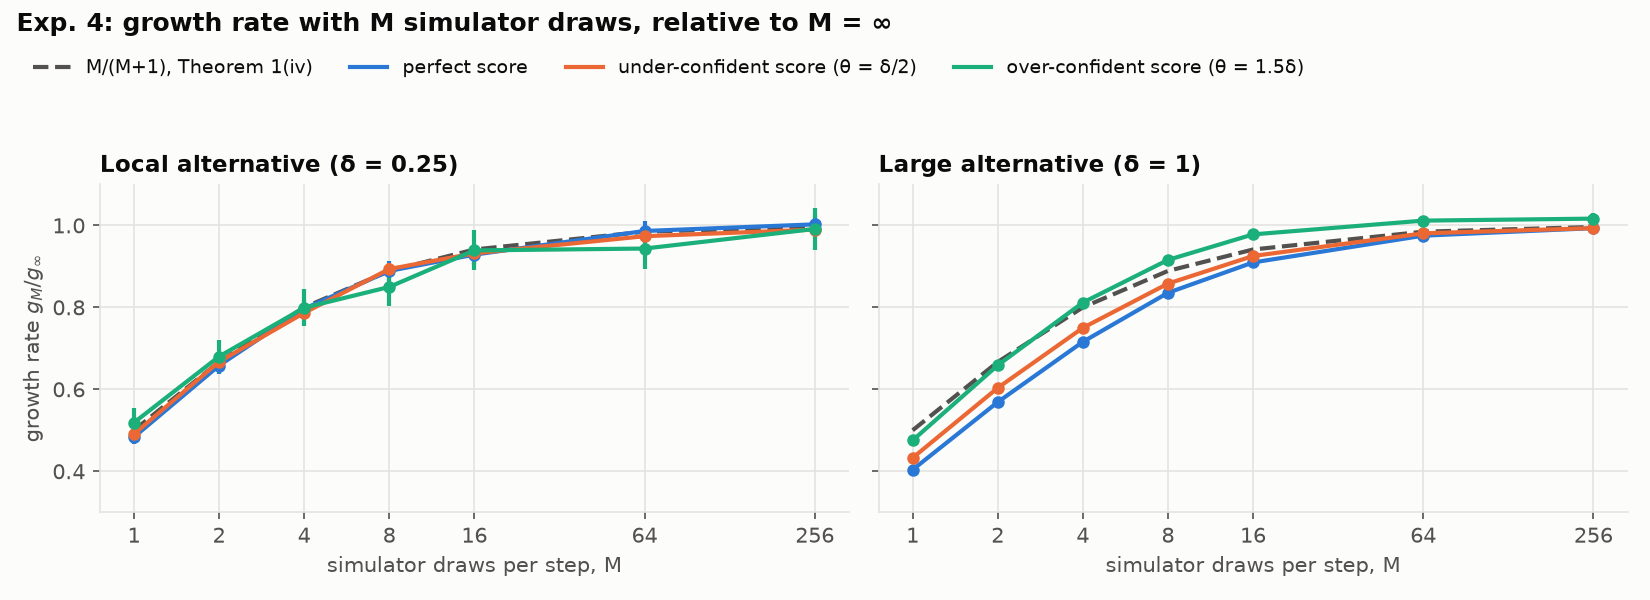
\includegraphics[width=\textwidth]{exp4_growth_rate.png}
\caption{Growth rate $g_M$ relative to $g_\infty$ for $P = \mathcal N(0,1)$,
$Q = \mathcal N(\delta, 1)$ and score $T(x) = e^{\theta x}$, estimated from
$4 \times 10^5$ draws (two standard errors shown). Dashed: $M/(M+1)$ from
Theorem~\ref{thm:growth}(iv).}
\label{fig:growth}
\end{figure}

Third, Theorem~\ref{thm:simlik} is checked with the bounded features
$\phi(x) = (\mathrm{clip}(x, \pm 3), \mathrm{clip}(x^2 - 1, \pm 3))/3$ (so
$d = 2$ and $G = \sqrt 2$), a uniform prior on the disc of radius $D = 3$ and
$P = \mathcal N(0,1)$. The mixture $\bar W_t$ is computed exactly on a grid of
31\,000 points and the hindsight optimum by convex optimisation, for 12 paths
of each of four scenarios: the null, a mean shift, a scale change, and a drift
at $t = 500$. The bound holds on every path and at every time: at $t = 2000$ the largest
regret over all paths is 7.5, against a bound of 21.5 (Supplement,
Section~S4). The regret grows at the interior rate
$(d/2)\log t$, with slopes between 1.01 and 1.10 against $d/2 = 1$. Under the
null the log wealth decreases, and under the alternatives the monitor keeps
pace with the best fixed score chosen in hindsight, including after the change
point, where that score is itself a compromise between the two regimes.

\subsection{Update rules}\label{sec:exp-blr}

Table~\ref{tab:blr} compares, on the drift task and the bandit with identical
data, the refitted point estimate with three of the update rules of
Section~\ref{sec:predictive}, updated at every step with no burn-in. All are
valid, with false alarms between 1.0\% and 3.3\%, whereas using the logistic
posterior odds directly as the bet gives between 14\% and 74\%. The logistic
Bayesian learning rule with the probability-scale predictive $\kappa\bar\eta$
is the fastest on both tasks and makes the method insensitive to the
flexibility of the features: with degree-6 features its power is 0.97, against
0.84 for the refitted estimate. On the simulation likelihood, the
posterior-predictive bet beats the plug-in bet at the posterior mean (223
against 265 steps), as Proposition~\ref{prop:approx} suggests. The
predictive-first updates are valid and somewhat slower on the drift task, and
on par on the bandit. The Supplement (Section~S4) reports all variants,
including the ratio-scale predictive, the Bayesian-bootstrap forest and the
degree-6 features, with a discussion of why the learners differ.

\begin{table}[t]
\centering
\caption{Update rules, MC e-process throughout (400 replications). BLR: online
Bayesian learning rule (Section~\ref{sec:blr}) on the logistic loss with the
probability-scale predictive, or on the simulation likelihood with the
posterior-predictive mixture bet (prior variance 0.03); predictive update: the
predictive-first rule \eqref{eq:mp} on the simulation likelihood, averaged over
predictive-resampling paths. All variants are in the Supplement.}
\label{tab:blr}
\begin{tabular}{llrrr}
\toprule
task & score & false alarms & power & median stop \\
\midrule
drift & refitted point estimate & 0.030 & 0.990 & 198 \\
 & BLR, logistic & 0.018 & 0.983 & 209 \\
 & BLR, simulation likelihood & 0.013 & 0.968 & 223 \\
 & predictive update, simulation likelihood & 0.010 & 0.920 & 234 \\
bandit & refitted point estimate & 0.028 & 1.000 & 49 \\
 & BLR, logistic & 0.030 & 1.000 & 38 \\
 & predictive update, simulation likelihood & 0.013 & 1.000 & 57 \\
\bottomrule
\end{tabular}
\end{table}

The Supplement compares the Monte Carlo e-process with the Besag--Clifford
e-process of \citet{dombowsky2026besag} on the drift task, where the null is
i.i.d. When the likelihood ratio is available the Monte Carlo normalisation
costs almost nothing (median 36 steps against 35 for the exact oracle); knowing
the parametric family of the drift is worth a factor of about 3.5 over learning
it from samples (58 against 209 steps); and with a learned score all-in betting
fails (power 0.41), so the mixture over $\lambda$ is the right strategy.

\subsection{Comparison with concurrent methods}\label{sec:exp-concurrent}

The concurrent methods of Section~\ref{sec:intro} use the same bet and differ
from ours in how the score is chosen. We compare them on the drift task and the
bandit, with the same simulations, the same mixture over $\lambda$ and the same
data for every method, so that only the score differs. For
\citet{forre2026anytime} we use their two scores: the score refitted every ten
steps by maximising the penalised empirical growth on the past, which is the
maximiser of the simulation likelihood under a ridge penalty, with the bet
placed at the maximiser; and a score fitted once, before monitoring, on
simulations from a guessed alternative. For \citet{cortinovis2026slice} we use
SLICE as it would serve our question, with a single null ($G = 1$): an
amortised neural ratio network trained once on $2 \times 10^5$ simulations from
the simulator's parametrised family (curvature $b$ for the drift, a location
shift per arm for the bandit), evaluated at a predictable estimate of the
parameter. Both concurrent methods assume independent data; in the bandit they
are run on simulations under the arm actually chosen, which our
Theorem~\ref{thm:valid} makes valid, and once as published, with the twin run
on random arms. Besides the alternatives of Sections~\ref{sec:exp-drift}
and~\ref{sec:exp-bandit}, which lie inside SLICE's family, each task has an
alternative outside it: in the drift the curvature is unchanged and the first
coordinate is 20\% wider, and in the bandit the most pulled arm keeps its mean
and its noise is 50\% larger.

\sbox{\widetab}{\begin{tabular}{lrrrrrr}
\toprule
 & \multicolumn{2}{c}{drift} & \multicolumn{2}{c}{bandit} & false & time \\
score & in family & out of family & in family & out of family & alarms & (s) \\
\midrule
ours, BLR logistic & 0.98 (209) & 0.70 (344) & 1.00 (38) & 1.00 (112) & 1.8--2.0\% & 0.3 / 0.2 \\
ours, simulation likelihood & 0.97 (223) & 0.85 (258) & 1.00 (55) & 0.99 (157) & 1.0--1.3\% & 0.3 / 0.15 \\
F\&B, refitted on the past & 0.99 (200) & 0.89 (250) & 1.00 (61) & 0.99 (167) & 1.5--2.0\% & 1.0 / 0.65 \\
F\&B, fitted in advance & 1.00 (61) & 0.01 & -- & -- & 2.5\% & -- \\
SLICE, neural ratio, $G = 1$ & 1.00 (71) & 0.01 & 1.00 (35) & 0.56 (258) & 0.7--3.3\% & 0.45 / 0.4 \\
F\&B, twin on random arms & -- & -- & \multicolumn{2}{c}{false alarms 100\%} & -- & -- \\
\bottomrule
\end{tabular}}%
\begin{table}[t]
\centering
\caption{Comparison with the scores of \citet{forre2026anytime} (F\&B) and
\citet{cortinovis2026slice} (SLICE); 400 replications per scenario. Entries:
power within the horizon and, in brackets, the median stopping time;
``in family'': the alternatives of Sections~\ref{sec:exp-drift}
and~\ref{sec:exp-bandit}; ``out of family'': departures that SLICE's
parametrised family does not contain. False alarms: range over the two tasks.
Time: computing time per replication on one core, drift / bandit; the
simulators are cheap here, so it measures mostly the cost of the score, and
for SLICE it excludes the training of the network. The F\&B score fitted in advance uses the true in-family drift
alternative. All variants are in the Supplement.}
\label{tab:concurrent}
\small
\begin{tabular}{@{}c@{}}\resizebox{\textwidth}{!}{\usebox{\widetab}}\end{tabular}
\end{table}

Table~\ref{tab:concurrent} shows four things. First, conditioning on the action
is necessary for every score: run as published, with the twin on random arms,
the refitted score of \citet{forre2026anytime} rejects the true null in every
bandit run, and with simulations under the chosen arm it is valid. Second,
scores that know where the departure lies are fastest: when the alternative is
inside the family, SLICE stops after 71 steps on the drift and 35 on the bandit,
and a score fitted in advance on the true alternative after 61, against about
200 for scores learned from the data. Third, this knowledge is also their
weakness: out of the family, SLICE has power 0.01 on the drift and 0.56 on the
bandit, and a score fitted on the expected alternative has power 0.01, while
every score learned from real against simulated outcomes keeps its power.
Fourth, among the scores learned from the data, the refitted maximiser of
\citet{forre2026anytime} and our posterior-predictive updates perform alike,
slightly better for the refit on the drift and for ours on the bandit, but ours
cost a third as much and carry the pathwise guarantee of
Theorem~\ref{thm:simlik}, since they update one step per observation instead
of refitting on the whole history. The network of SLICE cost $2 \times 10^5$
simulations and 26 seconds here, because the simulators are cheap;
\citet{cortinovis2026slice} use $10^7$ simulations per model. When an amortised
score is available, nothing forces a choice: the average of its wealth and
ours is again a test martingale, which is close to the faster of the two when
the departure is inside the family and keeps power when it is not.

\begin{remark}[Inside and outside the family]\label{rem:family}
SLICE fixes a parametrised family $\{P_\theta\}$ of simulators, with the null
at $\theta_0$, and bets with the score
$s_t = \log (p_{\hat\theta_{t-1}}/p_{\theta_0})$, where $\hat\theta_{t-1}$ is
estimated from the past real outcomes; its tilted null is
$\tilde T_t = P_{\hat\theta_{t-1}}$. An alternative is \emph{inside the family}
when $Q = P_\theta$ for some $\theta \ne \theta_0$, and \emph{outside} it
otherwise. Outside, $\hat\theta_t$ converges to the projection
$\theta^* = \arg\min_\theta \KL(Q\|P_\theta)$, and with an unlimited budget
the growth rate tends to
$g_\infty = \KL(Q\|P_{\theta_0}) - \KL(Q\|P_{\theta^*})$
(Theorem~\ref{thm:growth}(ii)). When $\theta^* = \theta_0$ the score itself
tends to zero, every factor tends to one, and the wealth stops growing however
large $\KL(Q\|P_{\theta_0})$ is and however good the network.

Both out-of-family alternatives of Table~\ref{tab:concurrent} are of this
kind. In the drift, the family is $x = (z_1, z_2 + b(z_1^2 - 1))$ with
$z \sim \mathcal N(0, I)$, in which $x_1 \sim \mathcal N(0, 1)$ for every $b$,
and the real data are $x = (1.2 z_1, z_2 + b_0(1.44 z_1^2 - 1))$ with
$b_0 = 0.5$. No $b$ produces the wider first coordinate, and the
least-squares estimate of $b$ converges to
$\E[x_2(x_1^2 - 1)]/\E[(x_1^2 - 1)^2] = b_0$, so the power is 0.01. In the
bandit, the family is
$y \mid a = \mu_a + \delta_a + e^{\varepsilon/2} - e^{1/8}$ with
$\varepsilon \sim \mathcal N(0, 1)$, in which $\delta$ moves only the location
of each arm, while the real noise of the most pulled arm is 1.5 times larger
with the same mean. The estimate of $\delta_a$ converges to zero, and the
power of 0.56 comes only from its early fluctuations. Our scores
$z(x)^\top\theta$ are learned from real against simulated outcomes rather than
within a family of simulators, and their features contain $x_1^2$ and the
squared outcome of each arm, so a change of scale moves $\tilde T_t$ towards
$Q$; their power is 0.70 to 0.85 on the drift and 1.00 on the bandit.

Our network is trained as a binary classifier of joint against shuffled
pairs (NRE-A), whereas \citet{cortinovis2026slice} use the contrastive
estimator NRE-C \citep{miller2022contrastive}. Both estimate
$\log p_\theta(y)/m(y)$, NRE-C up to a function of $y$ alone, which cancels in
$s_t$. The choice can affect the power inside the family, where our network is
already close to the exact ratio (71 against 75 steps on the drift, 35 against
35 on the bandit), but not outside it, where the exact ratio itself has power
0.005 on the drift.
\end{remark}

The difference between the two scores learned from the data is also a
difference in what kind of predictive they are. The refitted score of
\citet{forre2026anytime} is a prequential forecasting system in the sense of
\citet{dawid1984present}: a sequence of one-step predictives
$\tilde T_t \propto p_t\, e^{\hat\theta_{t-1}^\top\phi}$, each computed from the
past, which is all that validity and the prequential reading of the wealth
\eqref{eq:prequential-wealth} require; the same holds for SLICE at its
estimated parameter. It is a plug-in, however. A sequence of plug-ins at a
refitted maximiser is in general not the predictive sequence of any
exchangeable model, so it has no de Finetti representation with a parameter
and a posterior \citep{fortini2000exchangeability,fortini2024exchangeability};
it is a martingale, the condition of \citet{fong2023martingale} and of
\citet{berti2004limit}, only approximately; and it carries no uncertainty about
the score's parameter. Our updates average over that uncertainty, through the
posterior of the simulation likelihood, which is an exact Bayesian predictive,
or through predictive resampling, under which the parameter of the
predictive-first rule \eqref{eq:mp} is an exact martingale. This averaging is
what yields the pathwise regret bound of Theorem~\ref{thm:simlik} and the
cautious early bets that make our scores competitive at a third of the cost.

\subsection{Auditing a language-model API with adaptively chosen prompts}\label{sec:exp-llm}

The comparison above isolates the score. The actions are the other half of
the method, and an audit of a language-model API shows what they add. An API
advertises a model $P$ and may answer some queries with a cheaper substitute.
The auditor can query the API and can run $P$ locally, but evaluates neither
likelihood. As in the routing audit of \citet{cortinovis2026slice}, the probes
are prompts that ask for random output, which each model answers in its own
reproducible way: eight random digits, an integer between 1 and 100, a colour,
and six coin flips. The advertised model is Qwen2.5-1.5B-Instruct
\citep{qwen2024qwen25} quantised at 8 bits; the substitutes are the same model
at 4 and 3 bits, and a different, smaller model, Qwen2.5-0.5B-Instruct. All
replies are real outputs, generated with \texttt{llama.cpp}
\citep{gerganov2023llamacpp} at temperature one, 3000 per prompt for $P$ and 1500 for each
substitute, and, as in \citet{cortinovis2026slice}, only the routing is
simulated. At each step the auditor chooses a prompt $A_t$, observes the API's reply $X_t$,
and draws $M = 8$ replies of $P$ to the same prompt. Under the null the real reply and
the simulations are drawn from the same pool of $P$'s replies, so they are
exactly exchangeable given the past.

The prompt is chosen by an upper confidence bound on the realised log growth
of each prompt, with each prompt kept above a tenth of the queries; the choice
depends on the past only, so Theorem~\ref{thm:valid} applies. The learned
score is a logistic BLR on hashed character $n$-grams, with one block of
weights per prompt. We compare it with SLICE, whose score
$\log\{1 - \hat\theta_t + \hat\theta_t\, r_k(y)/p_k(y)\}$ uses one routing
fraction $\theta$ for all prompts, and with a score fitted in advance, as in
\citet{forre2026anytime}, equal to the log-ratio $\log r_k/p_k$. Both are
given 500 replies per prompt of the 4-bit substitute, from which a classifier
estimates $r_k/p_k$ for each prompt $k$, and both are run, as published, on
prompts drawn uniformly at random. The routing sends 30\% of all queries to
the substitute, or 50\% of the colour and number queries only, which lies
outside SLICE's family; with the 3-bit and the 0.5B substitutes the
baselines' guess of the substitute is wrong.

\sbox{\widetab}{\begin{tabular}{lrrrrrrr}
\toprule
 & \multicolumn{2}{c}{as published, uniform} & \multicolumn{4}{c}{our design, adaptive} & uniform \\
\cmidrule(lr){2-3}\cmidrule(lr){4-7}\cmidrule(lr){8-8}
substitute, routing & SLICE & in advance & SLICE & in advance & average & learned & learned \\
\midrule
4-bit, all prompts & 82 & 44 & 71.5 & \textbf{40.5} & 50 & 220 (0.94) & 249 (0.71) \\
4-bit, two prompts & 76 & 39 & 57 & \textbf{30} & 39 & 134 (0.99) & 227 (0.86) \\
3-bit, all prompts & 149 (0.96) & 72 & 109 (0.97) & \textbf{50} & 65.5 & 160 (0.98) & 204 (0.94) \\
0.5B, all prompts & 110 (0.99) & 70 & 95 & \textbf{48} & 56 & 109 & 123 \\
0.5B, two prompts & 107 & 59 & 57 & \textbf{23} & 29 & 52 & 77 \\
\bottomrule
\end{tabular}}%
\begin{table}[t]
\centering
\caption{Auditing a language-model API (Section~\ref{sec:exp-llm}): median
number of queries to an alarm, over the runs that reject within 400 queries,
with the power when below one; 400 replications. ``In advance'': the score
fitted in advance as in \citet{forre2026anytime}, on the 4-bit substitute;
``average'': the average of its wealth and the learned score's. False alarms
under the null: 0.0\% (SLICE, both designs), 3.5\% and 2.5\% (fitted in
advance, published and adaptive), 2.8\% (average), 3.5\% and 2.0\% (learned
score, adaptive and uniform); a twin that answers a random
prompt instead of the chosen one raises a false alarm in every run.}
\label{tab:llm}
\small
\setlength{\tabcolsep}{4pt}
\begin{tabular}{@{}c@{}}\resizebox{\textwidth}{!}{\usebox{\widetab}}\end{tabular}
\end{table}

Table~\ref{tab:llm} shows three things. First, adaptive prompts help every
score. With prompts chosen from the past and the twin run on the chosen
prompt, both published scores need fewer queries than in their published
form in every scenario: SLICE from 107 to 57 and the score fitted in advance
from 59 to 23 when the routing depends on the prompt, and from 110 to 95 and
from 70 to 48 when the substitute is not the expected one. The learned score
gains up to 0.23 in power over uniform prompts. The auditor
moves towards the colour prompt, on which the substitutes differ most from
$P$, with up to 42\% of the queries. Second, validity requires the conditioning: the
same design with a twin that answers a random prompt rejects the true null
in every run (Proposition~\ref{prop:necessary}), while all conditioned
monitors keep false alarms below 5\%. Third, prior knowledge of the
substitute pays when it is right, and the learned score needs none: without
any reply of the substitute, the learned score with adaptive prompts matches
SLICE on the 0.5B substitute and needs half as many queries when the routing
depends on the prompt. The average of the two wealths, a test martingale by
construction, needs at most 16 queries more than the score fitted in advance
in our design, is faster than both published methods in three of the five
scenarios and ties in a fourth, and, being at least half the learned wealth,
keeps the learned score's power, up to a factor two in the threshold, however
wrong the guess of the substitute. The design is
semi-synthetic and the models are small; the replies, however, are real, and
the auditor needs only the ability to run the advertised model.

\paragraph{Computational cost.} The cost of the audit is the cost of the
simulator. Each step needs $M = 8$ replies of $P$, which take 2 to 8 seconds
on four CPU cores, while computing the bet and updating the score takes about
1.3~ms with the learned score ($d = 129$ weights), 1.1~ms with the score fitted
in advance, 1.6 to 1.8~ms with SLICE and 2.6~ms for the average of two
wealths. The e-process itself is therefore below 0.1\% of the running time
for every method, and what matters is the number of queries to an alarm,
which the adaptive choice of prompts reduces by up to 61\%. The methods
differ in their fixed and growing costs. Ours needs nothing before monitoring
but 200 replies of the twin to standardise the features, and its update costs
the same at every step, $O(d^3)$ for the Gaussian update as implemented,
$O(d^2)$ with rank-one updates, so the total cost is linear in the number of
steps. The score fitted in advance and SLICE need replies of a guessed
substitute before monitoring, 500 per prompt here, or, for an amortised
network, simulations across the simulator's family, $2 \times 10^5$ in
Section~\ref{sec:exp-concurrent} and of the order of $10^7$ in
\citet{cortinovis2026slice}. SLICE's estimate of the routing fraction and the
refit of \citet{forre2026anytime} revisit the whole history at each update,
so their cost per step grows with $t$, unless sufficient statistics are
available; on the drift task the refit costs about three times our update
(Table~\ref{tab:concurrent}). These timings are of our implementations, not
the authors'.

%======================================================================
\section{A multi-arm multi-stage trial designed in silico}\label{sec:trial}
%======================================================================

\subsection{The trial and its twin}\label{sec:application}

Automated insulin delivery for type~1 diabetes doses insulin from the readings
of a continuous glucose monitor (CGM). Dosing algorithms are designed and tested
on the UVA/Padova type~1 diabetes simulator
\citep{dallaman2007meal,kovatchev2009insilico,dallaman2014uva}, which the US Food
and Drug Administration accepted as a substitute for animal trials in
preclinical testing \citep{kovatchev2009insilico}, and the same simulator is
used to design clinical trials of dosing strategies: arms are compared in
silico, and the simulator's predictions justify the design. We use the
open-source implementation \texttt{simglucose} \citep{xie2018simglucose} of its
2008 academic version, a 13-dimensional ordinary differential equation model
of meal absorption, glucose kinetics, hepatic glucose production and
subcutaneous insulin absorption, through a vectorised port that reproduces
\texttt{simglucose}'s trajectories to within $5 \times 10^{-4}$~mg/dL. Four
sources of randomness make it a stochastic simulator: insulin sensitivity
fluctuates within every five-minute interval (the parameters $V_{mx}$ and
$k_{p3}$ are multiplied by $e^{0.15\eta}$), carbohydrate absorption varies
($C$ grams are absorbed as $Ce^{0.2\eta}$), and the CGM has the Johnson-$S_U$
error of \citet{breton2008analysis}. The physiological state is hidden and the
per-interval perturbations enter the dynamics nonlinearly, so the law of a
day's CGM trace has no tractable density: the setting of this paper, in which
the simulator can only be sampled.

We consider a MAMS trial of five strategies run by the pump in closed loop:
\begin{itemize}
  \item \textbf{A, control:} carbohydrate bolus, correction to 140~mg/dL above
        150, basal suspended below 80;
  \item \textbf{B, aggressive:} bolus $\times 1.5$, correction to 100, suspend
        below 60;
  \item \textbf{C, conservative:} bolus $\times 0.8$, correction to 160, suspend
        below 90;
  \item \textbf{D, intensified:} bolus $\times 1.2$, correction to 120, suspend
        below 70;
  \item \textbf{E, tight correction:} bolus $\times 1.0$, correction to 110,
        suspend below 80.
\end{itemize}
The outcome is the time in range (70--180~mg/dL) over a full day, 06:00 to
06:00, with meals of 50, 70 and 80~g at 07:00, 12:30 and 19:00. According to
the simulator, arms B and C are worse than control (time in range 0.79 and 0.84
against 0.91) and arms D and E are equivalent to it (0.90 and 0.91). The trial
has three stages. In each, 50 new participants, each one of the ten adult
virtual patients drawn at random, are allocated in permuted blocks among the
arms still active, and every participant already enrolled is observed for one
more day. Participants carry their physiological state from one day to the
next, so a participant's day depends on their earlier treatment. After stages
1 and 2 an interim analysis compares each active experimental arm with control
on all participant-days so far and drops it for futility when $z < -1$ (first
interim) or $z < 0$ (second). Participants on a dropped arm are re-assigned to
the active experimental arm with the highest interim time in range, or to
control if none is left, and new participants are allocated only to active
arms. The trial has 150 participants and 300 participant-days, and every
element of the design, which arm a participant receives, on which day and
after which history, is chosen from the data.

The twin is the in-silico trial itself: for each participant-day, the
simulator with that participant's parameters is re-initialised at the
participant's current physiological state and run $M = 16$ times under the arm
assigned for that day. Participant-days are monitored in a fixed order within
each stage, and the score is the logistic BLR predictive of Section~\ref{sec:blr}
on six summaries of the day relative to the twin's noise-free path (mean and
standard deviation of the residual, time below 70 and above 180~mg/dL, and the
arm), with interactions between the arm and the residual and time-below-range
features. We compare it with four alternatives: the plug-in bet on the same
score; a \emph{stateless} twin, run under the assigned arm but started from the
resting state, which ignores the participant's history and therefore the
consequences of earlier treatment and re-assignment; a \emph{pooled} twin,
started from rest under an arm drawn uniformly from the five, which is the
pre-trial in-silico prediction and ignores both the allocation and the history;
and a $t$-test of standardised time-in-range residuals recomputed after every
participant-day. A single alarm says that the twin fails somewhere, but a trial
team needs to know under which arm. We therefore also run one e-process per arm,
each with its own score, which bets only on that arm's participant-days and has
factor one otherwise. Whether a participant-day is spent on arm $k$ is decided
before its outcome, so by Theorem~\ref{thm:valid} each is a test martingale for
the hypothesis that the twin is correct under arm $k$, whatever the interim
decisions and re-assignments. Each arm's e-value is its wealth at the end of the
trial, or when it first reaches $K/\alpha$ with $K = 5$, and e-BH
\citep{wang2022false} is applied across the arms. This is the bandit
multiple-testing construction of \citet{xu2021unified} with the twin as the
null; e-BH controls the false discovery rate under the arbitrary dependence
between arms that the shared interim decisions create.

Under the null, the participants are the simulator. We consider two
departures. Under \emph{insulin resistance}, insulin sensitivity is 25\% lower
than in the virtual cohort, in every arm. Under \emph{defensive snacking},
participants told that their regimen is intensified (arms B and D) eat an
unannounced 20~g snack at bedtime against night-time lows. The simulator does
not know this, and arms A, C and E remain exactly as the twin predicts, so the
false discovery rate of e-BH is well defined.

\subsection{Results}

\sbox{\widetab}{\begin{tabular}{lrrr}
\toprule
monitor & null & insulin resistance & defensive snacking \\
\midrule
MC e-process, twin at the participant's state & 0.02 & 1.00 (4) & 0.99 (32) \\
plug-in bet & 0.47 & 1.00 (5) & 1.00 (28) \\
stateless twin (ignores the history) & 0.95 & 1.00 (4) & 1.00 (33) \\
pooled twin (ignores allocation and history) & 1.00 & 1.00 (8) & 1.00 (58) \\
$t$-test, recomputed & 0.46 & 1.00 (17) & 1.00 (22) \\
\midrule
\multicolumn{4}{l}{\emph{design: share of trials with the arm active at the end}} \\
B / C / D / E & 0.00 / 0.01 / 0.27 / 0.50 & 1.00 / 0.00 / 1.00 / 0.79 & 0.02 / 0.01 / 0.93 / 0.42 \\
participants re-assigned (mean) & 65 & 14 & 43 \\
\midrule
\multicolumn{4}{l}{\emph{per-arm e-processes and e-BH: share of trials in which each arm is flagged}} \\
A / B / C / D / E & 0 / 0 / 0 / 0 / 0.01 & 1 / 1 / 1 / 1 / 1 & 0 / 0.64 / 0 / 0.99 / 0.01 \\
\bottomrule
\end{tabular}}%
\begin{table}[t]
\centering
\caption{A three-stage MAMS trial with futility analyses and re-assignment,
checked against its in-silico twin (150 participants, 300 participant-days,
100 replications per scenario). Top: rejection rate by the end of the trial
and, in brackets, the median number of participant-days before the first
alarm. Middle: the design, as the share of trials in which each arm is still
active at the end, and the mean number of re-assigned participants. Bottom:
share of trials in which e-BH flags each arm, at $\alpha = 0.05$.}
\label{tab:trial}
\begin{tabular}{@{}c@{}}\resizebox{\textwidth}{!}{\usebox{\widetab}}\end{tabular}
\end{table}

Table~\ref{tab:trial} summarises 100 replications of each scenario. Only the
monitor that conditions on both the allocation and the history is valid, with a
false-alarm rate of 2\%. The stateless twin raises a false alarm in 95\% of
trials: after the first day participants no longer start from rest, and after a
re-assignment their state reflects a treatment they no longer receive. The
pooled twin, the pre-trial prediction, rejects a true null in every trial, and
the recomputed $t$-test and the plug-in bet raise false alarms in 46\% and 47\%
of trials. Both parts of the conditioning are therefore necessary, on the
action and on the history, and the alternatives' alarms under the departures
carry no evidence.

Insulin resistance is detected in every trial after a median of four
participant-days, and the design reacts to it: arms B and D, which compensate
for resistance, survive every interim, and C is dropped. Defensive snacking is
detected in 99\% of trials after a median of 32 participant-days, and it changes
the design as well. The snack protects the intensified arm D from night-time
lows, so D survives to the end in 93\% of trials instead of 27\% under the null
and receives 41\% of all participant-days instead of 17\%: the trial favours an
arm for a reason that its in-silico justification does not contain. e-BH
names the arm. Under the null it flags some arm in 1\% of trials, under
resistance all five arms in every trial, and under snacking D in 99\% of trials
and B in 64\%, while A, C and E are flagged in at most 1\%, a false discovery
rate of 0.3\%. Arm B is found less often because the design usually drops it at
the first interim, after about ten participant-days: an arm that the trial
abandons accumulates little evidence, which is the price of a monitor that does
not influence the allocation. With the simulation-likelihood learner of
Section~\ref{sec:blr} (prior variance 0.03) instead of the logistic one, the
conclusions are the same but detection is slower: false alarms stay at 2\%
(98\% and 100\% for the stateless and pooled twins), snacking is detected in
99\% of trials after a median of 51 participant-days instead of 32, and e-BH
flags D in 99\% of trials and B in 39\%, with no false discovery.
The predictive-first learners and the Bayesian-bootstrap forest are valid as
well, with false alarms in 1--5\% of trials, against 81--98\% for the stateless
twin, and detect snacking in 99\% of trials (Supplement, Section~S4).

Two caveats matter in practice. The twin is re-initialised at the participant's
true physiological state, which is observable in silico but would have to be
estimated from CGM and insulin records in a real trial; sampling from the
twin's filtering distribution instead breaks exact exchangeability, and the
guarantees of \citet{barber2026montecarlo} for approximately exchangeable
samples are the natural tool. And an alarm says that the in-silico
justification of the design has failed, not that an arm is unsafe or
ineffective; in a trial it would be reported to the data monitoring committee,
and its consequences for the trial's efficacy analysis, which is not the object
of this monitor, are for the design to specify. A simpler single-stage,
three-arm version with Thompson-sampling allocation, and the monitoring of a
single patient under closed-loop control, are in the Supplement and lead to the
same conclusions.

%======================================================================
\section{Related work}\label{sec:related}
%======================================================================

Classical Monte Carlo tests compare a fixed dataset with simulations from the
null \citep{besag1989generalized}; \citet{fischer2024sequential} make them
anytime-valid in the number of simulations for a fixed dataset, and
\citet{barber2026montecarlo} give guarantees without exact joint
exchangeability. Here the data themselves arrive over time, and fresh
simulations are drawn for each new observation. The closest work is
\citet{dombowsky2026besag}, who normalise an arbitrary statistic into an
e-value with samples exchangeable with the data under the null, produced by
the parallel MCMC method of \citet{besag1989generalized} when the null can
only be sampled by MCMC. For the unnormalised likelihood ratio they show
log-optimality as $M \to \infty$ and a non-asymptotic lower bound on the
e-power, and they give composite nulls of finite cardinality, confidence
regions and a Besag--Clifford e-process for an i.i.d.\ stream, including a
plug-in score for a composite alternative. Relative to their work, this paper
adds actions chosen from the data, with the conditioning requirement and its
necessity; the analysis of learned scores through the tilted null and the local
efficiency $M/(M+1)$; the predictive view of the score and exact Bayesian
updating on the simulation likelihood with its pathwise regret; and per-arm
monitoring in adaptive designs. Their MCMC construction applies directly when
the simulator is itself an MCMC sampler.

Two concurrent papers use the same normalised bet for independent data.
\citet{forre2026anytime} test a simulator $P_0$ against an alternative $P_1$
that can also only be sampled, or against any departure from $P_0$. They show
that the likelihood ratio is the optimal score for every $M$, bound the loss
from a finite $M$, prove approximate growth optimality of scores fitted by
maximising the empirical growth, under compactness and M-estimation
conditions, and refit the score online on past observations; data streams that
depend on the past are left open. \citet{cortinovis2026slice} invert the
e-process over the parameter of a simulator into confidence sequences, with
amortised neural ratio scores trained before monitoring and fixed, and extend
validity to observations that depend on i.i.d.\ covariates; in an appendix
they note that the construction extends to dependent data when the
simulations are drawn conditionally on the observed history. Relative to both,
this paper develops that direction for actions chosen from the data and
simulators with state, gives the conditioning required under an arbitrary
allocation rule, shows that it is necessary and quantifies the failure
when it is dropped, reads arbitrary scores through the tilted null with the
local efficiency $M/(M+1)$, gives sequential Bayesian and predictive updates of
the score with a pathwise regret bound, and applies the method to adaptive
designs. Neither paper updates the score's parameter by Bayes' rule: both bet
at a point estimate, the maximiser of the empirical growth in
\citet{forre2026anytime} and a predictable estimate or posterior summary in
\citet{cortinovis2026slice}. Treating the bet as a likelihood, averaging it
over the posterior of the score's parameter, the prequential reading of the
wealth and the pathwise regret bound are specific to this paper.

Model-X sequential tests of conditional independence \citep{shaer2023modelx}
draw a dummy covariate from its known conditional law at each step and bet on a
learned predictor, the same mechanism as ours with $M = 1$ applied to a
different null. Sequential predictive two-sample tests bet with an online
classifier separating two streams
\citep{podkopaev2023sequential,shekhar2023nonparametric}, the sequential
kernelised Stein discrepancy tests goodness of fit when the score function is
available \citep{martinez2025sequential}, and conformal test martingales
\citep{vovk2003testing,vovk2021testing}, including weighted versions for
deployed AI systems \citep{prinster2025watch}, test the exchangeability of a
stream with no reference model. Randomisation tests and e-processes for
adaptively collected data \citep{nair2023randomization,zampieri2025sequential},
anytime-valid off-policy inference \citep{waudbysmith2024anytime} and adaptive
auditing of AI systems \citep{zhou2026adaptive} handle adaptivity, but none of
them uses a simulator as the null; digital-twin validation by re-initialising
the twin from observed states \citep{ghasemloo2026subtrace} uses the same
conditioning idea with fixed-sample tests. Prequential posteriors
\citep{sinharoy2026prequential} assimilate data into generative forecasting
models with intractable likelihoods through a scoring-rule loss estimated from
simulations, and target the parameter with the best one-step-ahead predictive
loss under misspecification; their aim is to calibrate the simulator, whereas
ours is to test it, and the simulation likelihood is the instance of their
construction, with the logarithmic loss of an exactly fair bet and learning
rate one, whose posterior mixture is a test martingale. In bandit multiple testing, one
e-process per arm combined by e-BH controls the false discovery rate under
arbitrary adaptive sampling \citep{xu2021unified}; there the hypotheses concern
the arms' effects and the sampling can be chosen to make the tests powerful,
whereas our per-arm monitors test the twin, with the allocation fixed by the
trial. Finally, reading the wealth as a prequential likelihood ratio follows
\citet{dawid1984present}; computing the marginal likelihood as a product of
one-step posterior predictives is Dawid's prequential form, the Bayes universal
code of minimum description length
\citep{rissanen1984universal,grunwald2007minimum}, and the basis of sequential
Monte Carlo estimates of the evidence \citep{kong1994sequential,chopin2002sequential},
and it is related to cross-validation by \citet{fong2020marginal}
(Section~\ref{sec:predictive}); the link between predictive scores and Bayes factors
is the prequential view of the marginal likelihood
\citep{clarke1990information}; taking the predictive sequence as the primitive
is the approach of martingale posteriors \citep{fong2023martingale}; and the
simulation likelihood connects the monitor to contrastive learning
\citep{oord2018representation,ma2018noise} and the score update to the Bayesian
learning rule \citep{khan2023bayesian,jones2024bong}.

%======================================================================
\section{Discussion}\label{sec:discussion}
%======================================================================

The Monte Carlo e-process separates two concerns that are usually entangled.
Validity comes from exchangeability with fresh, correctly conditioned
simulations, and holds for any score and any policy, including interim
analyses and re-assignments. Power comes from the score, which is a sequence of
one-step predictives; Theorem~\ref{thm:growth} measures it by the distance
between the tilted null and the truth, scaled by $M/(M+1)$, and
Theorem~\ref{thm:simlik} shows that exact Bayesian updating on the simulation
likelihood achieves the growth of the best score in a class, with no
recomputation. Approximations made when computing the score can therefore cost
power but never validity, and the score can be updated either through a
Gaussian approximation of a posterior or directly through its predictive, as
martingale posteriors do: in our experiments both routes are valid everywhere,
and the Gaussian route is usually faster because its covariance damps early
bets.

The actions are a source of power, not only a threat to validity. Once the
simulator is run under the action taken, the design may be chosen to gather
evidence where it accumulates fastest, and Theorem~\ref{thm:valid} keeps the
monitor valid whatever the rule. In the audit of Section~\ref{sec:exp-llm},
choosing the prompts adaptively makes every score faster, ours and the two
concurrent ones alike, by 8\% to 61\% in the number of queries. Methods built for
independent data and a fixed design, such as \citet{forre2026anytime} and
\citet{cortinovis2026slice}, gain from being placed in this design, and
without the conditioning on the action they lose validity altogether.

The concurrent methods and ours are therefore complementary rather than
competing. SLICE answers a different question, which values of a simulator's
parameter are compatible with the data, and its test of a single null is a
by-product. When the departure lies inside the simulator's parametrised family
it is the fastest method we compared (Section~\ref{sec:exp-concurrent}); when
it does not, its power depends on where the departure projects onto the
family, and it vanishes when the projection is the null itself, however
accurate the network (Remark~\ref{rem:family}). It also needs the family and
an amortised training on simulations from it, of the order of $10^7$ in
\citet{cortinovis2026slice}. A score learned from real against simulated
outcomes needs neither, and pays for this with a slower start when prior
knowledge of the alternative exists: in the audit, a score fitted in advance
on the right substitute stops after 30 to 41 queries, the learned score after
134 to 220. The natural synthesis is to use an amortised or pretrained score
as the centre of the prior of the online update, rather than as a separate
bet. The monitor would then start as fast as the pretrained score and correct
it where the guess is wrong, with the validity of Theorem~\ref{thm:valid}
and the pathwise guarantee of Theorem~\ref{thm:simlik} relative to that
prior. The average of the two wealths used in Section~\ref{sec:exp-llm} is a
cruder version of this synthesis, and already within 16 queries of the faster
of its two components.

Several limitations remain. The null is a simple conditional null; simulators
with unknown calibration parameters need composite-null constructions, such as
universal inference or reverse information projections \citep{grunwald2024safe},
adapted to samplers. MCMC-based samplers and estimated initial states break
exact exchangeability, and the guarantees of \citet{barber2026montecarlo}
suggest how to control the resulting error. Theorem~\ref{thm:simlik} compares
the monitor with the best score in a parametric class, not with the true
density ratio, and its regret bound is not known to be optimal; the
approximate one-step update used in practice is covered only through
Proposition~\ref{prop:approx}, and in our experiments the logistic learner,
which has no such guarantee, is more powerful than the simulation-likelihood
learner that has one: by 7\% in stopping time on the drift task and by about
60\% in the trial, because the latter's bets are too cautious. Closing this gap,
for instance with a tempered or sharper posterior that keeps the guarantee, is
the most useful next step. Finally, the experiments are
low-dimensional; high-dimensional simulators call for learned feature maps and
structured posterior approximations. High-energy physics is a natural target,
since searches for new physics already compare collision data with large
samples from the Standard Model simulator using learned classifiers
\citep{dagnolo2019learning}, and the Monte Carlo e-process would make such
comparisons anytime-valid as data accumulate.



\backmatter

\bmhead{Supplementary information}
The online supplement contains three further analyses (a single patient under
closed-loop control, a single-stage response-adaptive trial, and a comparison
with the Besag--Clifford e-process) and additional results for Sections 5
and 6.

\bmhead{Acknowledgements}
% TO BE COMPLETED BY THE AUTHOR. Check the journal's policy on generative-AI
% tools; if it requires disclosure, state here how such tools were used.
[To be completed.]

\section*{Declarations}

\begin{itemize}
\item \textbf{Funding.} [To be completed.]
\item \textbf{Competing interests.} The author has no competing interests to
declare.
\item \textbf{Ethics approval and consent to participate.} Not applicable.
\item \textbf{Consent for publication.} Not applicable.
\item \textbf{Data availability.} No external data are used. The replies of the language models in
Section~\ref{sec:exp-llm} were generated with the code below from the publicly
released Qwen2.5 models and are in the \texttt{data} folder of the code
repository; all other data are simulated by the code below.
\item \textbf{Materials availability.} Not applicable.
\item \textbf{Code availability.} All methods, experiments, tables and figures are implemented in Python and
available at \url{https://github.com/elenabortolato/evalues4generative}. The
file \texttt{REPRODUCIBILITY.md} in that repository lists, for every table
and figure, the script and command that produce it, the output file and an
indication of the running time. Every replication is seeded, so the reported
numbers are reproduced exactly with the stated library versions.
\item \textbf{Author contribution.} The author is the sole contributor.
\end{itemize}

\begin{appendices}
%======================================================================
\section{Notation}\label{app:notation}

\sbox{\widetab}{\begin{tabular}{lll}
\toprule
symbol & meaning & where \\
\midrule
$t$, $\F_t$, $\G_t = \F_{t-1} \vee \sigma(A_t)$ & time; information after step $t$; information when the bet at $t$ is placed & Sec.~\ref{sec:setting} \\
$A_t$, $a$ & action chosen by the design (arm, dose, prompt) & Sec.~\ref{sec:setting} \\
$X_t$ & real outcome at time $t$ & Sec.~\ref{sec:setting} \\
$Y_{t,1}, \ldots, Y_{t,M}$; $M$ & simulator draws under $A_t$ from the current state; their number & \eqref{eq:mc} \\
$U_{t,0}, \ldots, U_{t,M}$ & pooled outcomes $(X_t, Y_{t,1}, \ldots, Y_{t,M})$ & Sec.~\ref{sec:simlik} \\
$H_0$ & the simulator reproduces the conditional law under the actions taken & Sec.~\ref{sec:setting} \\
\midrule
$P_t$, $p_t$ & simulator law and density of the next outcome (the null) & Sec.~\ref{sec:setting} \\
$Q_t$, $q_t$ & true law and density of the next real outcome & Sec.~\ref{sec:power} \\
$\tilde T_t$ & tilted null of the score (its forecast), with density $T_t p_t / Z_t$ & \eqref{eq:tilt} \\
$Q_\theta$, $q_\theta$ & model for the truth: the tilt of $P$ by $\theta^\top\phi$ & Sec.~\ref{sec:exactbayes} \\
$\pi_0$, $\pi_t$ & prior and posterior on $\theta$ & Sec.~\ref{sec:exactbayes} \\
$m_t$; $m(x_{1:t})$; $\tilde m_t$, $\tilde m(x_{1:t})$ & posterior predictive; marginal likelihood; their SMC estimates & \eqref{eq:prequential} \\
$\nu_t = \mathcal N(\bar\theta_t, S_t^{-1})$ & Gaussian approximation of the posterior (BLR) & \eqref{eq:blr} \\
$P_a$, $\bar P$ & law under action $a$; action-ignoring simulator law & Prop.~\ref{prop:necessary} \\
$\mathbb P_n$ & empirical predictive & Sec.~\ref{sec:blr} \\
\midrule
$s_t$, $T_t = e^{s_t}$ & score, chosen from $\G_t$ & \eqref{eq:mc} \\
$Z_t$; $\widehat Z_t$; $Z(\theta)$ & $\E_{P_t}[T_t]$; its Monte Carlo estimate; $\E_P[e^{\theta^\top\phi}]$ & \eqref{eq:tilt} \\
$B$ & bound on the score, $|s_t| \le B$ & Cor.~\ref{cor:cumulative} \\
$E_t$; $E^{(M)}$; $E_t^\infty$ & Monte Carlo factor; the same in the one-step analysis; its limit as $M \to \infty$ & \eqref{eq:mc} \\
$E_t(\theta)$; $\bar E_t$; $E_t^{\nu}$ & factor of the score $\theta^\top\phi_t$; posterior mixture; mixture under $\nu_{t-1}$ & Sec.~\ref{sec:simlik} \\
$\lambda$, $\Lambda$; $\alpha$ & betting fraction and its grid; level & \eqref{eq:wealth} \\
$W_t$; $\bar W_t$ & wealth; mixture wealth over $\theta$ & \eqref{eq:wealth} \\
\midrule
$g_M = g_M(Q, P, T)$; $g_M(\lambda)$ & growth rate with $M$ simulations; with fraction $\lambda$ & \eqref{eq:growthrate} \\
$g_{M,t}$; $g_\infty$ & conditional growth rate at $t$; limit as $M \to \infty$ & \eqref{eq:growthrate} \\
$\rho$ & $\E_Q[T]/Z$ & Thm.~\ref{thm:growth} \\
$\varepsilon$, $\psi$, $h$, $\tilde h$ & local alternative $dQ/dP = 1 + \varepsilon\psi$; score $T = e^{\varepsilon h}$; $h - \E_P h$ & Thm.~\ref{thm:growth} \\
$R_a$ & likelihood ratio $dP_a/d\bar P$ & Prop.~\ref{prop:necessary} \\
$\varpi_a$; $u_b$; $K$ & long-run fraction of steps playing $a$; weights of a randomised twin; number of arms & Cor.~\ref{cor:falsealarm} \\
\midrule
$\theta$, $\phi_t$, $z(x)$, $d$ & parameter; features; standardised features; dimension & Sec.~\ref{sec:simlik} \\
$\Theta$, $D$, $G$; $L_t(\theta)$ & parameter set, its diameter, feature bound; simulation likelihood & Thm.~\ref{thm:simlik} \\
$\bar\theta_t$, $S_t$; $\Sigma_t$ & mean and precision of $\nu_t$; covariance of an approximate posterior & \eqref{eq:blr} \\
$\bar\eta$, $v$, $\kappa$ & predictive mean and variance of the logit $z^\top\theta$; $(1 + \pi v/8)^{-1/2}$ & Sec.~\ref{sec:blr} \\
$\ell_t$, $\nabla_t$, $J_t$; $I_t$ & per-step loss, its gradient and Fisher information; accumulated information & \eqref{eq:mp} \\
$c_t(x)$ & classifier probability $\sigma(z(x)^\top\theta_t)$ (predictive-first rule) & Sec.~\ref{sec:algorithm} \\
$w_k$ & weights of the outcomes: one for $X_t$, $1/M$ for each $Y_{t,j}$ & Sec.~\ref{sec:algorithm} \\
$\mathcal U_t$ & update rule of the predictive & Sec.~\ref{sec:scores} \\
$N$; $h_{\max}$ & number of trees, posterior nodes or resampling paths; truncation & Sec.~\ref{sec:blr} \\
\midrule
$\KL$, $\chi^2$, $D_2$ & Kullback--Leibler, chi-squared and Rényi-2 divergences & Sec.~\ref{sec:power} \\
\bottomrule
\end{tabular}}%
\begin{table}[h]
\centering
\caption{Notation. Laws are written with fixed letters: $P$ for the
simulator, $Q$ for the truth, $\tilde T$ for the tilted null of a score $T$ and $m$ for
a Bayesian posterior predictive; lower-case letters are densities, except that
$\tilde T$ denotes both the tilted null and its density $T p/Z$; $\tilde m$
denotes sequential Monte Carlo estimates.}
\label{tab:notation}
\begin{tabular}{@{}c@{}}\resizebox{\textwidth}{!}{\usebox{\widetab}}\end{tabular}
\end{table}

\section{Proofs}\label{app:proofs}
%======================================================================

We work conditionally on $\G_t$, so the score is fixed, and write
$\E_{Q\otimes P^M}$ when $X \sim Q$ and $Y_1, \ldots, Y_M$ are i.i.d.\ $P$,
independent of $X$. Two facts recur: $\E_{P\otimes P^M}[E^{(M)}] = 1$
(Proposition~\ref{prop:exact}), and the change of measure
$\E_{Q\otimes P^M}[f/(dQ/dP)(X)] = \E_{P\otimes P^M}[f]$.

\paragraph{Proof of Theorem~\ref{thm:growth}.}
Let $V = \sum_{j \le M} T(Y_j)$, $E^{(M)} = (M+1)T(X)/\{T(X)+V\}$ and
$E^\infty = T(X)/Z = (d\tilde T/dP)(X)$, so that $g_\infty = \E_Q[\log E^\infty]$.

(i) By Jensen's inequality and the change of measure,
\[
\begin{aligned}
g_M - \KL(Q\|P) = \E_{Q \otimes P^M}\Big[\log\frac{E^{(M)}}{(dQ/dP)(X)}\Big]
&\le \log \E_{Q \otimes P^M}\Big[\frac{E^{(M)}}{(dQ/dP)(X)}\Big] \\
&= \log \E_{P \otimes P^M}\big[E^{(M)}\big] = 0 .
\end{aligned}
\]

(ii) $V/M \to Z$ almost surely, so
$E^{(M)} = \frac{M+1}{M}\,T(X)/\{T(X)/M + V/M\} \to E^\infty$. If $|s| \le B$,
$T(X)$ and $\{T(X)+V\}/(M+1)$ lie in $[e^{-B}, e^{B}]$, so
$|\log E^{(M)}| \le 2B$ and dominated convergence gives $g_M \to g_\infty$.
Taking $\E_Q$ in $\log(d\tilde T/dP) = \log(dQ/dP) - \log(dQ/d\tilde T)$ gives
$g_\infty = \KL(Q\|P) - \KL(Q\|\tilde T)$.

(iii) $\log E^\infty - \log E^{(M)} = \log[\{T(X) + V\}/\{(M+1)Z\}]$. Jensen over
$Y_{1:M}$, with $\E[V] = MZ$, then over $X \sim Q$, with $\E_Q[T]/Z = \rho$:
\[
g_\infty - g_M \le \E_Q\log\Big(1 + \frac{T(X)/Z - 1}{M+1}\Big)
\le \log\Big(1 + \frac{\rho - 1}{M+1}\Big) \le \frac{\rho-1}{M+1}.
\]
This is Theorem~3 of \citet{dombowsky2026besag}.

(iv) Take $\varepsilon < 1/\|\psi\|_\infty$. Let $U_0 = X$, $U_k = Y_k$, and
$\bar h$, $\overline{h^2}$ the averages of $h(U_k)$, $h(U_k)^2$ over
$k = 0, \ldots, M$. Expanding the log of the average of $e^{\varepsilon h(U_k)}$,
with a remainder $R$, $|R| \le C\varepsilon^3\|h\|_\infty^3$ uniformly in the sample,
\[
\log E^{(M)} = \varepsilon h(X) - \log\frac{\sum_k e^{\varepsilon h(U_k)}}{M+1}
= \varepsilon\big(h(X) - \bar h\big) - \frac{\varepsilon^2}{2}\big(\overline{h^2} - \bar h^2\big) - R .
\]
Under $Q \otimes P^M$: $\E[h(X) - \bar h] = \frac{M}{M+1}(\E_Q h - \E_P h)
= \frac{M}{M+1}\varepsilon\E_P[\tilde h\psi]$, since $dQ/dP = 1+\varepsilon\psi$
and $\E_P\psi = 0$; the empirical variance $\overline{h^2} - \bar h^2 \in [0, \|h\|_\infty^2]$
has mean $\frac{M}{M+1}\E_P[\tilde h^2]$ under $P \otimes P^M$, and
$\frac{M}{M+1}\E_P[\tilde h^2] + O(\varepsilon)$ under $Q \otimes P^M$; and
$\E[R] = O(\varepsilon^3)$. Hence
\[
g_M = \frac{M}{M+1}\,\varepsilon^2\Big(\E_P[\tilde h\psi] - \tfrac12\E_P[\tilde h^2]\Big) + O(\varepsilon^3),
\]
and $\E_P[\psi^2] - \E_P[(\psi - \tilde h)^2] = 2\E_P[\tilde h\psi] - \E_P[\tilde h^2]$.
Finally $\KL(Q\|P) = \E_P[(1 + \varepsilon\psi)\log(1 + \varepsilon\psi)]
= \frac{\varepsilon^2}{2}\E_P[\psi^2] + O(\varepsilon^3)$.

\paragraph{Proof of Proposition~\ref{prop:necessary}.}
Given $\G_t$, $T$ is fixed, $X \sim P_a$ and $Y_1, \ldots, Y_M$ are i.i.d.\
$\bar P$. Let $B = \sup T$, $Z = \E_{\bar P}[T] > 0$ and
$\bar T_M = M^{-1}\sum_j T(Y_j)$.

(i) Dividing by $M$,
\[
E_t = \frac{M+1}{M}\cdot\frac{T(X)}{T(X)/M + \bar T_M} \to \frac{T(X)}{Z}
\quad\text{almost surely},
\]
since $(M+1)/M \to 1$, $T(X)/M \to 0$ and $\bar T_M \to Z > 0$ by the strong law.
For the means, let $G_M = \{\bar T_M \ge Z/2\}$. On $G_M$, the denominator is at
least $\bar T_M \ge Z/2$, $T(X) \le B$ and $(M+1)/M \le 2$, so
$E_t \le 2B/(Z/2) = 4B/Z$, and
dominated convergence gives $\E[E_t^k\mathbf 1_{G_M}] \to \E_{P_a}[T^k]/Z^k$,
$k = 1, 2$. On $G_M^c$, $E_t \le M+1$, and Hoeffding's inequality
\citep{hoeffding1963probability} gives $P(G_M^c) \le e^{-MZ^2/(2B^2)}$, so
$\E[E_t^k\mathbf 1_{G_M^c}] \le (M+1)^k e^{-MZ^2/(2B^2)} \to 0$.

(ii) If $P_a \ne \bar P$, some $A$ has $P_a(A) > \bar P(A)$ (otherwise the
inequality for $A$ and $A^c$ forces equality), and $T = 1 + \mathbf 1_A$ has
limit $\{1 + P_a(A)\}/\{1 + \bar P(A)\} > 1$. With $R_a = dP_a/d\bar P$,
$\E_{P_a}[R_a] = \int R_a^2\, d\bar P$ and
\[
\chi^2(P_a\|\bar P) = \int (R_a - 1)^2\, d\bar P = \int R_a^2\, d\bar P - 1 .
\]
If $R_a$ is bounded and bounded away from zero, $T = R_a$ has limit
$1 + \chi^2$. Otherwise $T_c = \min(R_a, c) + 1/c \in [1/c, c + 1/c]$, and by
monotone convergence $\E_{\bar P}[T_c] \to 1$ and $\E_{P_a}[T_c] \to \int R_a^2\, d\bar P$,
so the limit for $T_c$ tends to $1 + \chi^2$.

(iii) Let $\xi_i = \log(1 - \lambda + \lambda E_i)$, which lies in an interval of
length $C$ since $0 < E_i \le M+1$. As $\log(1+x) \ge x - 2x^2$ for $x \ge -1/2$
(Taylor), with $x = \lambda(E_i - 1)$, on $\Omega_0$ and for $i \ge t_0$,
\[
\E[\xi_i \mid \G_i] \ge \lambda\mu - 2\lambda^2\sigma^2 \ge \lambda\mu/2 .
\]
$\Delta_i = \xi_i - \E[\xi_i \mid \G_i]$ are martingale differences for
$(\G_{i+1})$ with $|\Delta_i| \le C$, so Azuma--Hoeffding
\citep{azuma1967weighted} and Borel--Cantelli give $t^{-1}\sum_{i \le t}\Delta_i \to 0$
almost surely. Since $W_t \ge |\Lambda|^{-1}\exp(\sum_{i \le t}\xi_i)$,
\[
\frac{\log W_t}{t} \ge -\frac{\log|\Lambda|}{t} + \frac1t\sum_{i < t_0} \xi_i
+ \frac1t\sum_{t_0 \le i \le t} \big(\E[\xi_i \mid \G_i] + \Delta_i\big),
\]
whose $\liminf$ on $\Omega_0$ is at least $\lambda\mu/2$.

\paragraph{Proof of Corollary~\ref{cor:falsealarm}.}
(i) When $a$ is played, $X \sim P_a$ and the draws are i.i.d.\ $\bar P$, so
Theorem~\ref{thm:growth}(ii)--(iii) applies with $Q = P_a$, $P = \bar P$
($\rho_a < \infty$ as $T$ is bounded). The laws do not change, so
$t^{-1}\sum_{i \le t}\E[\log E_i \mid \G_i] \to \sum_a \varpi_a g_M(a)$, and
Corollary~\ref{cor:cumulative} applies.

(ii) As in Theorem~\ref{thm:growth}(i), with $R_a = dP_a/d\bar P$ and
$e_\lambda = 1 - \lambda + \lambda E_t$,
\[
\E_{P_a \otimes \bar P^M}[\log e_\lambda] - \KL(P_a\|\bar P)
\le \log \E_{\bar P \otimes \bar P^M}[e_\lambda] = 0,
\]
and $\KL(P_a\|\bar P) \le \log\E_{P_a}[R_a] = \log\{1 + \chi^2(P_a\|\bar P)\}$ by
Jensen. Since $|s| \le B$ keeps $\log e_\lambda$ bounded, the martingale strong
law bounds each of the $|\Lambda|$ products, and hence $W_t$. For the
likelihood-ratio score $\tilde T_a = P_a$.

(iii) $\bar P(A) \ge u_a P_a(A)$ for all $A$, so $R_a \le 1/u_a$, which bounds
$\KL = \E_{P_a}[\log R_a]$ and $1 + \chi^2 = \E_{P_a}[R_a]$.

\paragraph{Proof of Proposition~\ref{prop:bayes}.}
With $q_\theta = dQ_\theta/dP$, $\E_P[q_\theta] = 1$, so by Fubini
$Z = \E_P[T_t] = 1$ and $E_t^\infty = T_t(X_t)$. Since
\[
T_t(x) = \frac{\int q_\theta(x) \prod_{i<t} q_\theta(X_i)\,\pi_0(d\theta)}
{\int \prod_{i<t} q_\theta(X_i)\,\pi_0(d\theta)},
\]
the product $\prod_{i \le t} T_i(X_i)$ telescopes to
$\int \prod_{i \le t} q_\theta(X_i)\,\pi_0(d\theta)$. The expansion is
\citet{clarke1990information}, and $\E_Q[\log q_\theta] = \KL(Q\|P) - \KL(Q\|Q_\theta)$.

\paragraph{Proof of Theorem~\ref{thm:simlik}.}
(i) Since $L_t = L_{t-1}E_t$ and $\pi_{t-1} \propto L_{t-1}\pi_0$,
$\int L_t\, d\pi_0 = \int L_{t-1}\,d\pi_0 \cdot \bar E_t$, and by induction
$\int L_t\,d\pi_0 = \prod_{i \le t}\bar E_i = \bar W_t$. As $\pi_{t-1}$ is
$\G_t$-measurable, Theorem~\ref{thm:valid} and Fubini give
$\E[\bar E_t \mid \G_t] = \int \E[E_t(\theta) \mid \G_t]\,\pi_{t-1}(d\theta) = 1$.

(ii) $F = \log L_t$ is concave: each $\log E_i(\theta)$ is linear minus a
log-sum-exp, with gradient $\phi_i(U_{i,0}) - \sum_k w_{ik}\phi_i(U_{i,k})$ of norm
at most $2G$. Let $\theta^*$ maximise $F$ on $\Theta$; then
$F(\theta) \ge F(\theta^*) - 2Gt\|\theta - \theta^*\|$. The set
$S_r = \theta^* + \frac{r}{2D}(\Theta - \theta^*) \subseteq \Theta$, $0 < r \le 2D$,
lies within distance $r$ of $\theta^*$ and has $\pi_0(S_r) = (r/2D)^d$, so
\[
\log \bar W_t \ge \log\int_{S_r} e^{F}\, d\pi_0 \ge F(\theta^*) - 2Gtr + d \log\frac{r}{2D},
\]
and $r = d/(2Gt)$ gives the first bound. For an interior maximiser, the
Hessian of $F$ is minus a sum of covariances of vectors of norm at most $G$, so
$F(\theta) \ge F(\theta^*) - \frac{tG^2}{2}\|\theta-\theta^*\|^2$ on the ball $B_r$,
with $\pi_0(B_r) \ge (r/2D)^d$; then
$\log \bar W_t \ge F(\theta^*) - \frac{tG^2 r^2}{2} + d\log\frac{r}{2D}$, and
$r = \sqrt{d/(tG^2)}$ gives the second bound.

(iii) Let $B_\Theta = \max_\Theta\|\theta\|$. For fixed $\theta$, $E_i(\theta)$
lies in $[(M+1)/(1 + M e^{2GB_\Theta}),\, M+1]$, so
\[
t^{-1}\textstyle\sum_{i\le t}\{\log E_i(\theta) - g_{M,i}(\theta)\} \to 0
\]
almost surely, as in
Proposition~\ref{prop:necessary}(iii). By (ii),
$\log \bar W_t \ge \sum_{i \le t} \log E_i(\theta) - d\log t - O(1)$. In the
i.i.d.\ case a countable dense subset of $\Theta$ and the continuity of $g_M$
give the supremum, and the last inequality is Theorem~\ref{thm:growth}(ii)--(iii)
for the score $e^{\theta^\top\phi}$.

%======================================================================
\section{Experimental details}\label{app:details}
%======================================================================

\paragraph{Refitted learner.} Balanced logistic regression on standardised
monomials of the observation (degree 4 or 6; for the bandit, per-arm terms
$1, y, y^2$), with a ridge penalty on all coefficients except the intercept.
It is refitted by eight Newton steps on all real observations and up to the
last 4000 simulator draws, every ten steps from step 20; until the first fit
the score is zero and $E_t = 1$.

\paragraph{Logistic BLR.} The same model, with prior $\mathcal N(0, I)$ on the
standardised coefficients and variance 10 on the intercept. Features are
standardised with 2000 (bandit: 3000) simulator draws from a stream
independent of the data. At each step the real observation has weight one and
each of the $M$ simulator draws weight $1/M$, and expectations under the
current posterior use the probit approximation. Scores are clipped to
$[-30, 30]$.

\paragraph{Simulation-likelihood BLR.} Prior $\mathcal N(0, \tau I)$ on the
standardised coefficients (no intercept, which cancels in $E_t(\theta)$), with
$\tau = 1$ or $\tau = 0.03$; the latter was chosen on 24 alternative runs of the
drift task, which are among the 400 reported. Expectations under the Gaussian
posterior use 32 fixed antithetic nodes $m + L\xi_s$ with $LL^\top = S^{-1}$,
and the bet is the average of $E_t(\theta)$ over the nodes.

\paragraph{Seeds and cost.} Replication $i$ uses seed $i$ under the null and
$10^6 + i$ under the alternative, for every method, so methods are compared on
identical real data. On four cores, the drift experiment takes about one minute
per 400 replications, and the MAMS trial about nine minutes per 100 replications of
one scenario.

%======================================================================
\section{Timing relative to concurrent work}\label{app:timeline}
%======================================================================

The manuscript was in preparation when \citet{forre2026anytime} (arXiv,
6~October 2026) and \citet{cortinovis2026slice} (arXiv, October 2026)
appeared. The conditioned Monte Carlo e-process, the bandit and multi-arm
multi-stage trial experiments, the simulation likelihood with
Theorem~\ref{thm:simlik}, and the per-arm e-BH procedure are recorded in the
version history of the code repository from 29 and 30 September 2026. Both
preprints develop the method for independent data;
\citet[Appendix~C.1.1]{cortinovis2026slice} note the possibility of
conditioning on the past for dependent data. The treatment of actions chosen
from the data and of simulators with state, the necessity of the conditioning
and the use of adaptive actions as a source of power are developed here. The comparisons with both papers in
Sections~\ref{sec:exp-concurrent} and~\ref{sec:exp-llm}, and the remarks
attributing shared results to them, were added after they appeared.
\end{appendices}

\bibliography{references}

\end{document}
